\documentclass[]{msulabm}
\usepackage[utf8]{inputenc}
\usepackage{amsmath}
\usepackage{graphicx}
%\usepackage[linktocpage]{hyperref}  % if not using colorlinks, use linktocpage
\usepackage[colorlinks]{hyperref}  % if not using colorlinks, use linktocpage
\usepackage{bm}            % bold math
\usepackage{multirow}
\usepackage[table]{xcolor} % provide alternating rows with colors
\usepackage{textcomp}
\usepackage{xfrac} % gives split-level fractions with '\sfrac{a}{b}
\usepackage{multicol}
\usepackage[section]{placeins} % provides \FloatBarrier, to keep floats from crossing this barrier
\usepackage{amssymb}
\usepackage{wrapfig} % provides wrapping figures with text.
%\usepackage{enumitem} % gives \begin{enumerate}[resume] to resume counting from previous enumerate
%\usepackage{subfigure}
%\usepackage{tikz} % to draw arrows
\usepackage{xtab} % provides xtabular, tabular environment that spans multiple pages and other awesome things
\usepackage[style=phys,biblabel=brackets,pageranges=false]{biblatex}
\usepackage{pdflscape}
\usepackage{ragged2e}
\usepackage{longtable}
\usepackage{mathabx} % gives astronomy symbols like \Earth
\usepackage{pdfpages}
\usepackage{wasysym}

\bibliography{references-manual,bbarker-zotero}

\newcommand{\abs}[1]{\left\lvert#1\right\rvert}

\title{Laboratory Manual}
\author{PHSC 12610 Black Holes \\ \\ The University of Chicago}
\date{Winter 2019}

\pagestyle{ruled}

\definecolor{lgray}{rgb}{.2,.2,.2}

\makeevenfoot{ruled}{\thepage}{\footnotesize{\textit{Last updated \today}}}{}
%\makeevenfoot{ruled}{\thepage}{}}{}
\makeoddfoot{ruled}{}{\color{lgray} \tiny{This work is licensed under \href{http://creativecommons.org/licenses/by-sa/4.0/}{CC BY-SA 4.0} by \href{mailto:bbarker@uchicago.edu}{the University of Chicago}.}}{\thepage}


% allows us to use subcaptions from the memoir class in figures. See Memoir Section 10.9
\newsubfloat{figure}

% don't worry so much about filling every page.
%\raggedbottom

% raise the penalty for splitting footnotes across different pages. Default is 100.
\interfootnotelinepenalty=10000

%\includeonly{amplifier/amplifier} 

% creates a standard length to use 
\newlength{\answerskip}
%\setlength{\answerskip}{90pt} 

%% use plus / minus if latex is squeezing the answer space too much
\setlength{\answerskip}{2cm plus 0.2cm minus 0.2cm}

\newlength{\qaskip}
\setlength{\qaskip}{\answerskip}
\addtolength{\qaskip}{\baselineskip}

% reduce vertical space between chapters in table of contents. Default is 2em.
\setlength{\cftbeforechapterskip}{1em}

% allow for extra line on a page to help prevent widow/orphan lines.
\sloppybottom

% Now we can caption a table outside of the table float environment (good for multi-page tables)
\newfixedcaption{\freetabcaption}{table}

%\includeonly{snells-law/snells-law}
%\includeonly{ohms-law/ohms-law}

\begin{document}
\maxtocdepth{chapter}

 % start roman numbering
 \frontmatter

\maketitle

%\clearpage

%Brent W. Barker

%Department of Astronomy \& Astrophysics

%The University of Chicago

%5640 South Ellis Ave.

%Chicago, IL 60637

%\href{mailto:bbarker@uchicago.edu}{bbarker@uchicago.edu}

%\vspace{2\baselineskip}

%\includegraphics{cc-by-sa-88x31}

%\textcopyright{} 2018 Brent W. Barker. Except where otherwise noted, this work is copyrighted under the Creative Commons Attribution-ShareAlike International 4.0 License. To view a copy of this license, visit \url{http://creativecommons.org/licenses/by-sa/4.0/}.

%\vspace{\baselineskip}

%These labs, excluding "Impulse and Momentum" and the appendices, are a derivative of "\href{https://%sites.google.com/site/scientificabilities/ISLE-labs}{ISLE Labs}" by the Rutgers Physics and Astronomy %Education Research group, used under the Creative Commons Attribution International 4.0 License.
%To view a copy of this license, visit \url{http://creativecommons.org/licenses/by/4.0/}.

%At Rutgers University, many people contributed to this project over the years.
%The list of names is very long and includes: Eugenia Etkina, Alan Van Heuvelen, Suzanne Brahmia, David %Brookes, Michael Gentile, Anna Karelina, Michael Lawrence, Marina Milner-Bolotin, Sahana Murthy, Maria %Ruibal-Villasenor, Aaron Warren, Xueli Zou.

 % skip to next right leaf (``recto'')
 \cleartorecto

 % the star means that the ToC itself is not listed in the ToC
 \tableofcontents*

 % start arabic numbering
\mainmatter 

\chapter{Behavior of gravity waves in water (the ripple tank)}\label{cha:ripple-tank}

%TODO include theoretical limit considerations in curve fitting

\section{Introduction}

The Michelson interferometer, named after University of Chicago professor Albert A. Michelson (Nobel prize in Physics 1907), is an extremely sensitive instrument capable of measuring incredibly tiny displacements.
A modern version of the Michelson interferometer has been developed by The Laser Interferometer Gravitational-Wave Observatory (LIGO) experiment to detect changes in distance of $10^{-19}\:$m (much less than the size of the nucleus of an atom!).
This displacement is sensed between mirrors separated by 4 km (see Figure~\ref{rt:fig:ligo-aerial}). There are two sites for LIGO --- one in Hanford, WA and the other in Livingston, LA.
The LIGO interferometer has recently detected gravitational waves for the first time (September 15, 2015); the first announced gravitational wave detection fits, with remarkable precision, the expected signal from the merging of two black holes, 29 and 36 solar masses, located 410 Mpc away.
The reported signal and the comparison to the fitted model are shown in Figure~\ref{rt:fig:ligo-signals}.

\begin{figure}
	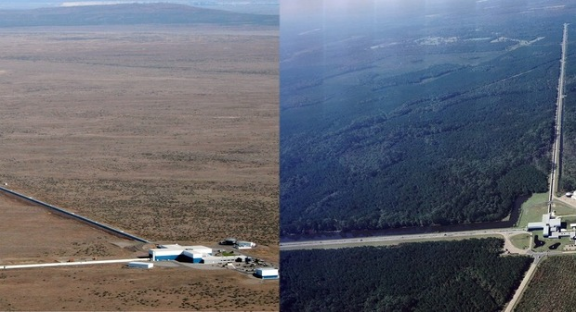
\includegraphics[width=\textwidth]{ripple-tank/ligo-aerial.png}
	\caption{An aerial view of the two LIGO sites.}\label{rt:fig:ligo-aerial}
\end{figure}

\begin{figure}
	\centering
	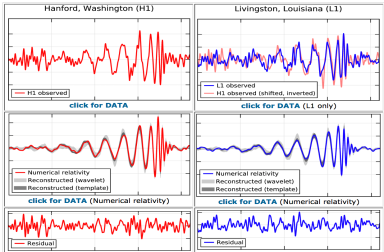
\includegraphics[width=0.7\textwidth]{ripple-tank/ligo-signals.png}
	\caption{The left panels show the LIGO signal at the Hanford site (top) and the best-fit model
		(middle) and the residual of the model minus the data (bottom). The residuals are consistent
		with noise. The right panels show the same for the Livingston site, with the Hanford signal
		plotted in red in the top panel to demonstrate the similarity of the two measurements (as
		expected in the event of a true gravitational wave signal). This first LIGO detection of a
		gravitational wave event marks a significant transformation in our collective ability to
		measure and understand black holes, and since that first detection, more black hole merger
		events have been detected and reported.}\label{rt:fig:ligo-signals}
\end{figure}

The working principle of the Michelson interferometer is the interference of light.
In this lab, you will first explore the concepts of interference with waves produced in water, in a device known as a ripple tank.
In particular, in this first portion of the lab you will experimentally verify a relationship between wave frequency and wavelength, and then demonstrate constructive and destructive wave interference.
You will then extend that understanding of interference to a wave geometry more appropriate to the second portion of the lab.
The final measurement with the ripple tank will allow you to show that plane waves propagating through a slit behave as though the slit were a new source of waves, propagating radially (i.e.\ in a circular pattern).

Next week, you will measure interference phenomena with light, with a modern version of the famous double-slit experiment performed by Thomas Young in 1801.
You will show that the interference properties of waves established in the first section of the lab apply to light as well, thus experimentally demonstrating that light behaves in a wavelike manner.

Having established the wavelike nature of light, you will then finally use a table-top Michelson interferometer to measure changes in distances smaller than a human hair (not quite LIGO sensitivity, but still pretty impressive!).

\section{Learning Goals}

\begin{itemize}
	\item Learn how to conduct an observational experiment, including collecting data and analyzing the data to find and describe a pattern quantitatively.
	
	\item Discover the relationship between frequency and wavelength of waves.
	
	\item Learn how to conduct a testing experiment, including identifying a hypothesis, designing an experiment, making a prediction, and comparing it to an experimental outcome.
	
	\item Gain familiarity with wave interference.
\end{itemize}

\section{An aside: picking a project topic}

By the end of lab today, ensure that you have chosen a topic for your presentation+paper project, and that it has been approved by your TA.

\section{The Scientific Cycle\protect\footnote{adapted from \cite{etkina_college_2014}}}

One way of describing science is the process of incrementally improving a shared model of how our universe works. In different fields of science, different methods and cycles are used, so there is no ``One True Scientific Method.'' One can still create a model for the process of science, and we describe here one such cycle (the hypothetico-deductive cycle), summarized in Figure~\ref{me:fig:isle}.

In this cycle, there are three types of experiments, each one representing a different stage of the scientific effort. One stage, often started when encountering a novel phenomenon, is the \textbf{observational experiment}. This is an experiment that consists of deciding what to observe and how to observe it, collecting data, finding a pattern, and brainstorming possible explanations for what is observed (also called ``hypotheses'').

Once one has some trial explanations, one can test one or more of those with a \textbf{testing experiment}. Here, one designs a new experimental procedure and uses each hypothesis to predict what will happen. Then the prediction is compared to the procedure's outcome. If they are different, then the hypothesis is judged to be not a helpful explanation for that phenomenon. If they are the same, then it is still helpful. Throughout this stage, one may make various assumptions that would need to be validated, as they can effect the prediction or outcome.

Once a hypothesis has been tested enough for people to find it useful, then it can be applied to solve practical problems, or to determine properties of particular situations, in an ``application experiment.''

\begin{figure}
	\centering
	\includegraphics[width=0.7\textwidth]{ripple-tank/islegraphic.png}
	\caption{A model of the process some scientists go through to create knowledge.\cite{etkina_millikan_2015}}\label{me:fig:isle}
\end{figure}

\section{Experiment 1: Observation of frequency and wavelength}

\textbf{Goal:} Observe gravity waves in a ripple tank and determine a mathematical relationship between frequency and wavelength.

\textbf{Available equipment:} ripple tank with strobe light and ripple generator, plane wave attachment, 2 dippers (narrow plastic rods), 1 short wall, 1 medium wall, 2 long walls for ripple tank, flashlights or desk lamps, digital camera (e.g.\ your smartphone), computer with ImageJ installed (can be your device), object of known size to be submerged

\begin{framed}
	\textbf{Caution: Flickering Lights!} You will be using a stroboscopic light in this lab. Such light is known to trigger reactions in some individuals (e.g. photosensitive epilepsy).
	If you are worried that you may be sensitive to strobe light, speak to the TA and skip attending this part of the lab.
	In any case, avoid staring directly at the light.
\end{framed}

\begin{framed}
	\textbf{Self-assessment:} To help you improve your scientific abilities, we provide you with self-assessment rubrics.
	A rubric is a scoring system.
	Self-assessment is determining how well you performed a particular task.
	So, these self-assessment rubrics are designed to help you evaluate your performance while you are designing and performing your experiment.
	
	The complete set of rubrics is available in Appendix~\ref{cha:rubrics}.
	In each lab, your report will be assessed using Rubric F, found in Table~\ref{rubric:f}, as well as 5 additional rubric rows listed in that lab.
	Each week, read through these and use them to evaluate your work as you design and perform the experiment.
	Your instructor will use the same rubrics to determine part of your grade for the lab.
\end{framed}	

\textbf{Rubrics to focus on during this experiment:} B7, B8, F1, F2. See Appendix~\ref{cha:rubrics} for details.

\subsection{The ripple tank and generator}

In this section you will explore interference phenomena using a ripple tank. The tank --- 42.5 cm x 42.5 cm and 2.5
cm deep --- is filled with water, and is equipped with a ripple generator. The generator uses voice coil actuators to
produce the precise and quiet up-and-down motion of the rippler arms. Waves are generated in the tank by the moving
dippers that touch the surface of the water. The generator also controls a light source that produces a bright, clear
image of the wave patterns in the ripple tank. The light can be used as a steady source or as a strobe to ‘freeze’ the
motion of the wave patterns (in this case the flashing light and the generator are driven with the same frequency). The
ripple generator frequency ranges from 1.0 to 50 Hz adjustable in 0.1 Hz increments. You will work with frequencies in
the range 16--32 Hz. A mirror placed below the tank and working in conjunction with a projection screen provide a
magnified image of the wave patterns in the water; you will record patterns seen on this screen by photographing them
with a digital camera. The ripple generator terminates in a bar with numerous clips in which you can place various
``dippers''.

\subsection{Suggestions for your experiment}

\begin{enumerate}
	\item You may want to decide on roles for each group member. Example roles include Facilitator (ensures time and group focus are efficiently used), Scribe (ensures work is recorded), Technician (oversees apparatus assembly, usage), Skeptic (ensures group is questioning itself). Note that each role is responsible for ensuring that the thing happens, rather than necessarily doing it themselves. \textbf{Decide if you are using these roles, and if so, assign them and note them in the lab report.}
	
	\item Ensure that every group member knows what the terms frequency and wavelength mean, in relation to waves. Use whatever means at your disposal to do this.
	
	\item This is an ``observational experiment.'' Review Rubric B (Table~\ref{rubric:b}) and discuss any unclear expectations with your group and the instructor. Note that your lab report will be graded, in part, on demonstration of Abilities B7 and B8.
	
	\item Ensure that one of the ripple tank's ripple generator is set up with 1 dipper fixed in the center clip of the bar that extends from the box, and that the height of the generator is such that the dipper just touches the top of the water. You can make coarse adjustments by moving the generator along the support rod, and fine adjustments with the two red knobs on it.
	
	\item Brainstorm different methods you could use to determine the relationship between wavelength and frequency. Feel free to play with the ripple tank as you do so, seeing what the frequency and amplitude knobs do. Notice that for different frequencies, different amplitudes produce the clearest image. Here are some things to consider:
	\begin{itemize}
		\item Which variable will you control (and thus will be the independent variable) and which will you measure?
		
		\item What is the range of the independent variable that you will use? How many different settings will you choose?
		
		\item You will need to use several settings of the independent variable, and then plot the data in a graph, decide on what pattern you see, and give some justification for that pattern. You can use words like ``proportional'', ``linear'', ``parabolic'', ``exponential'', ``logarithmic'', and so on, if they fit. Ensure you use the mathematical definition of these.
		
		\item How will you measure the wavelength?
		\begin{itemize}
			\item Is it a more precise measurement if you measure several of them at once and divide to get a single wavelength?
			
			\item The reflected image might magnify the ripple tank, so it can be helpful to place an object of known size in the tank, like a coin, so you can determine the correct scaling.
		\end{itemize}
		
		One way to take careful measurements of the wavelength is to take a picture of the projected tank, then use a program like ImageJ to measure the lengths you need. If you do so, one way to keep track of what settings go with what image is to mark a card with the settings and place it in view of the camera. See the section below on measuring lengths with ImageJ.
	\end{itemize}

	\item Decide on your measurement and analysis method and discuss it with an instructor before you begin. They will help increase the chances that your method will lead to successful results, or at least that the unhelpful path that you choose will take a short enough amount of time for you to change it when you discover it does not work. We want you to have productive failure that you have time to learn from.
	
	\item Perform your experiment. Your lab report for this experiment should include:
	\begin{itemize}
		\item A labeled sketch or photo of the setup, and a description of the experimental procedure (see Rubric F1).
		
		\item A plot of wavelength vs. frequency (with the independent variable on the horizontal axis)
		
		\item A description of the pattern found. This can be done with a line (straight or curved) showing the pattern you see (either drawn manually or using the curve fitting function of the plotting program, e.g.\ LibreOffice Calc or Microsoft Excel) and with words describing what you found. (B7)
		
		\item An equation to represent the pattern. This can be taken from a curve fit or found by hand. Make sure there is some discussion of how well the equation agrees with the data, but you don't need to be very precise about it. (B8)
		
		\item A discussion of the findings of the experiment and why it's helpful (for you and/or for science) (F2)
	\end{itemize}

\end{enumerate}

\subsection{Measuring lengths using ImageJ}

ImageJ (\url{http://imagej.nih.gov/ij/download.html}), which is installed on the lab computers, is useful for measuring lengths in images. To do so, load your image, then follow these steps to calibrate the ruler --- that is, to tell ImageJ how long something is in the image, so it knows how many pixels correspond to what length).

\begin{enumerate}
	\item Start with an image that has an object in it that you know one of the lengths of (e.g.\ the length of side, or a diameter).
	
	\item Open that image in ImageJ.
	
	\item Select the icon with the straight line on it, and click and drag along the known length.
	
	\item From the drop-down menu, select ``Analyze'' $>$ ``Set Scale...''.
	
	\item Set ``Known distance'' to the value of the known length.
	
	\item Set ``Unit of length'' to the unit you are using, for example ``mm'' for millimeters.
	
	\item Record the pixel scale given at the bottom of the box for future use.
	
	\item Now when you use the straight line tool, it will give the length in physical units in ImageJ's toolbar.
\end{enumerate}

\section{Experiment 2: Testing the conditions for constructive interference}

\textbf{Goal:} Test the hypothesis that constructive interference between two waves occurs at positions where the distance from each source differs by a half-integer number of wavelengths, or
\begin{equation}
 \Delta d = (m+\frac{1}{2})\lambda \,,
\end{equation}
where $\Delta d$ is the ``path length difference'', $\lambda$ is the wavelength, and $m$ is any integer.

\textbf{Available equation:} Same as in the previous experiment.

\textbf{Setup:} Instead of 1 dipper, use two dippers mounted with 3 empty clips between them on the bar. Ask the TA for assistance in setting this up. Adjust so that the dippers are just resting in the surface of the water. Adjust the frequency and amplitude to get clear, sharp waves.

\textbf{Rubric rows to be assessed in this experiment:} C1, C4, C7, F1, F2. See Appendix~\ref{cha:rubrics} for details.

\subsection{Testing this hypothesis}

In general, one tests a hypothesis by using it to make a prediction about what will happen in a certain experimental procedure. With this hypothesis, it asserts a relationship between path length difference, wavelength, and constructive interference. But there are only certain points on the ripple tank image where it is easy to see constructive interference --- the bright spots at the intersection of waves originating from both sources. For an example, see Figure~\ref{rt:fig:interference-2d}.

\begin{figure}
	\centering
	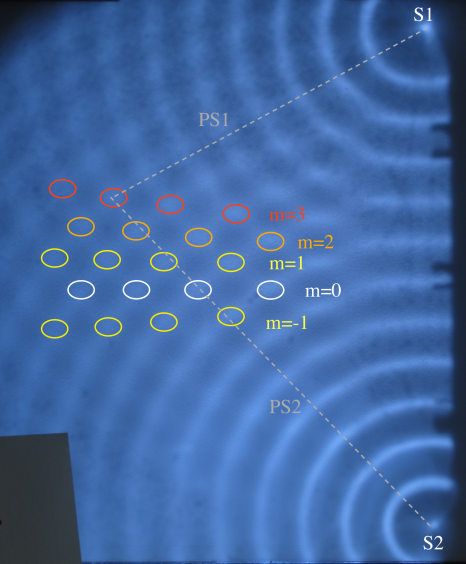
\includegraphics[width=0.7\textwidth]{ripple-tank/interference-2d.png}
	\caption{Example interference pattern for 2 dippers. The bright spots are circled. For a particular bright spot of constructive interference, the two path lengths PS1 and PS2 are drawn.}\label{rt:fig:interference-2d}
\end{figure}

In this case, it is easier to start by finding those locations, measuring the $\Delta d$, finding the wavelength for the given frequency using the relationship you found in Experiment 1, and solving for $m$. The hypothesis predicts that $m$ should always be an integer. As a result, your experiment becomes this: find out how close the experimentally determined $m$'s are to integers.

Brainstorm your experimental procedure, decide on it, discuss with your TA, then perform the experiment.

Your lab report for this experiment should include:
\begin{itemize}
	\item A clear description of the hypothesis (see Rubric C1).
	
	\item A labeled sketch or photo of the setup, and a description of the experimental procedure (F1).
	
	\item A clear statement of the prediction that the hypothesis makes for this particular procedure (C4).

	\item A table of path lengths, path length differences, and measured $m$ values.
	
	\item An analysis of how close the measured $m$ values are to the prediction. Use some quantitative measure of this, but don't worry about being precise about uncertainties (C7).
	
	\item A judgment about the hypothesis. Is it supported, disproved, or undetermined? (C8, though not assessed this time)
	
	\item A discussion of the findings of the experiment and why it's helpful (for you and/or for science) (F2).
\end{itemize}

%In the case of a hypothesis like this one, that includes a proposed equation, there is a useful template for coming up with a prediction:
%\begin{enumerate}
%	\item Note that this hypothesis is asserting that when the equation is true, there is constructive interference (a bright spot). So the goal is to test how true this is.
%	
%	\item Choose which variables you are holding constant, which one is the independent, and which is the dependent variable. In this case, you may not know what $m$ is ahead of time. You could choose it arbitrarily, for example $m=0$ first, and go from there.
%	
%	\item Once you decide on your procedure (which things to measure, how to vary the independent variable), you can use the equation to solve for the dependent variable, which becomes the prediction (Rubric C4).
%	
%	\item The set of dependent variables (for each chosen independent variable) becomes the prediction of the hypothesis that you will use to compare to experimental outcome (C7).
%\end{enumerate}
%
%\subsection{Suggestions for your experiment}
%
%\begin{itemize}
%	\item Note that constructive interference happens where there are bright spots in the projected image at the intersection of waves coming from both sources.
%	
%	\item There is an entire line of points that have the same path length difference from each source, so for each choice of $m$, there can be many 
%\end{itemize}

\section{Experiment 3: Observing plane waves encountering narrow gaps}

This experiment does not clearly follow the model of the scientific cycle, but is closest to an observational experiment. In next week's lab, you will investigate the properties of light traveling through small slits. Ripples in water are more obviously waves, so it is helpful to observe what happens here first.

Instead of dippers, remove them and position the bar so that it is resting in the water. This will produce straight line waves, or, in two dimensions, ``plane waves''. This is the same kind of waves we will use next week with light.

Adjust the amplitude and frequency, with the frequency in the range 20--25 Hz, until you see
clear well-defined vertical parallel lines. Now, insert the two large ``walls'' in the tank, parallel to the rippler bar and
perhaps 5cm away; allow a small (few mm) opening between the two wall sections, placed so that opening is vertically
centered in the projected image. Adjust the amplitude upward until you see a clear wave pattern radiating from that
opening. Take a picture. Repeat this with two apertures instead of one; do this by adding a smaller wall between the
two larger sections, with all sections parallel to the rippler bar, and a small gap between each larger wall and the central
smaller portion. Again, take a picture, adjusting amplitude as necessary to get well-defined waves.

The analysis of this will be done as individual homework.

\section{Individual Homework}

These questions are to be answered individually and your answers should be submitted under the Lab 1 Homework assignment on Canvas.

Both questions concern the last two situations recorded in the lab: the case of 2 walls (1 gap or ``aperture'') and the case with 3 walls (2 apertures).

\begin{enumerate}
	\item What wave pattern do you see in the case of a single aperture? What do you see In the case of a double aperture?
	How do these patterns compare to the data you took using dippers on the rippler bar?
	
	\item Is the wavelength of the pattern you observe consistent with the relationship between frequency and wavelength you
	measured with the dippers? Include any measurements and calculations you make in answering this question in your homework response, and be quantitative.
\end{enumerate}
\chapter{Behavior of electromagnetic waves in space (lasers and slits)}

% TODO include reason for different formula from previous lab with ripple tank

\section{Introduction}

In 1801, Thomas Young's ``double-slit'' experiment demonstrated the wave nature of light by showing that two coherent light sources produce interference patterns. You will perform a modern version of Young's experiment using a
laser as light source. The laser illuminates two thin slits, each of width $a$ separated by a distance $d$, which act as two
coherent sources of light. This is analogous to what you have observed with water waves in the previous lab section, in
which you saw a plane wave combined with an aperture (a slit) acting as a circular source of waves. An interference
pattern appears on a viewing screen, placed at a distance $L$ from the double slit, in the form of bright and dark regions
corresponding to maxima and minima of interference. You will use the interference pattern to measure the wavelength
$\lambda$ of the laser, and show that the same framework of equations that is derived in the introduction to the previous lab
holds for light too.

\section{Experiment 1: Observing patterns made by 1 and by 2 slits}\label{li:sec:exp1}

\textbf{Goal:} Describe the patterns made by a laser that is incident on 1 slit and on 2 slits, and the differences and similarities between them.

\textbf{Available equipment:} optical bench, viewing screen, blank white paper, PASCO ``Multiple Slits'' assembly, red laser with mounting clamp, support stand, optionally computer with ImageJ installed

\begin{framed}
	\textbf{Warning: Laser Hazard!} The power of our lasers is low enough that the normal human blink reflex is sufficient to protect against incidental eye exposure.
	
	That being said, the following rules reduce the risk of eye exposure to laser light:
	\begin{enumerate}
		\item Do not direct the laser beam into anyone's eye.
		\item Be aware of the laser reflecting off of mirror-like surfaces and where that beam goes.
		\item Turn off the laser when not in use.
		\item Keep the laser pointing horizontally and near the plane of the table, while keep your eyes above that plane.
		\item To determine whether the laser is on, put your hand or a light-colored object in front of the beam, rather than looking into the laser aperture.
	\end{enumerate}
\end{framed}

\textbf{Rubrics to be assessed for this section:} F1, F2. See Appendix~\ref{cha:rubrics} for details.

\subsection{Setup}
Ensure the red laser is turned on and pointed at the slit assembly. Rotate the head of the slit assembly so that the active slit is the ''Comparison'' slit location with both a single
and double slit furthest counter-clockwise. Adjust the laser so that the active slit
is well illuminated by the laser spot. Note the laser should be pointed slightly upward if the laser head is ~10cm off the
table, and pointed so it hits the screen ~5cm from the top edge, and so moving the slit assembly closer to the laser will
move the spot on the slit assembly lower, and moving it further will move the spot higher. With the slits aligned with the
laser, you will see light on the screen, but no longer a simple spot. Instead, you will see a vertical feature, the details of
which depend on whether the laser is illuminating the single slit, or the double slit. Nudge the rail end back and forth to
see the difference.

Include the following in your report:
\begin{enumerate}
	\item A labeled photo or sketch of the experimental setup.
	
	\item An image of each pattern from the first slit assembly setting, taken from the same camera location.
	
	\item A written description of each pattern and how they are alike and different. Do you see same pattern in the double slit as you do in the single slit (in addition to another pattern)?
	
	\item What happens to the double-slit image if the slit separation is wider, like in the second setting in the ``Comparisons'' section of the assembly?
	
	\item How about when the slits are wider, like in the third setting? 
\end{enumerate}

\section{Experiment 2: Testing the wave hypothesis}

\textbf{Goal:} Determine whether light can be described as a wave. Note that if this is true, then light from a laser would be a plane wave.



\textbf{Available equipment:} Same as in Section~\ref{li:sec:exp1}, plus a green laser with mounting clamp

\textbf{Rubrics to be assessed for this section:} C4, C7, C8, G2, G4, F1, F2. See Appendix~\ref{cha:rubrics} for details.

\subsection{Behavior of a plane wave incident on single and double slits}

The following equation describes the location, $y_m$ (measured relative to the center of the pattern), of the $m$th interference minimum (dark spot) seen on a screen when a plane wave is incident on a single slit.
\begin{equation}
y_m = \frac{m \lambda L}{a} \,,
\end{equation}
where $L$ is the distance from the slit to the screen, and $a$ is the width of the slit.

For a double slit, the following equation describes the location $y_n$ of the $n$th interference maximum (bright spot) seen on a screen when a plane wave is incident on a double slit.
\begin{equation}
y_n = \frac{n \lambda L}{d} \,,
\end{equation}
where $d$ is the distance between the two slits.

\subsection{Suggestions for your experiment}

\begin{itemize}
	
	\item \textbf{REQUIRED:} Use both the green laser and the red laser for this experiment, and ensure that you keep the data (image and setup parameters) for use in the individual homework.
	
	\item For measuring the interference minima and maxima, you can do so by putting a paper on the screen and marking the locations directly, then measuring the marks with a ruler or with ImageJ. You could also take a picture of the pattern directly. Ensure that you take a reference photo with a known length on the screen, and take the image as face-on as possible, from the same location every time if you are taking multiple images.
	
	\item The green laser has a wavelength of $532\:$nm. You can assume that this value is exact, with zero uncertainty.
	
	\item The stated uncertainty in the slit size and separation according to the manufacturer (PASCO) is $\pm$ 0.005 mm for the slit width ($a$), and $\pm$ 0.01 mm for the slit spacing ($d$).
	
	\item If you use a value with an uncertainty in a calculation, if you want to use that value for comparison, you must propagate the uncertainty through to the final value. See Appendix~\ref{unc:sec:prop}.
	
	\item To compare your outcomes to your predictions, get a value with uncertainty for each, then compare them using the $t'$ test, described in Section~\ref{unc:sec:comparing}.
\end{itemize}

\subsection{Items to include in your report}

Relevant rubric rows from Appendix~\ref{cha:rubrics} are listed in parentheses.

\begin{enumerate}
	\item Statement of the hypothesis (C1).

	\item Description of the experimental setup and procedure (C2, F1).
	
	\item The quantitative prediction that the hypothesis makes about what will happen during the experimental procedure (C4). Ensure that uncertainty is handled correctly (G2).
	
	\item A report of the experimental outcome (results), neatly organized (G4).
	
	\item Determination of whether / how much the prediction agrees with the outcome, comparing using uncertainties (C7, G2).
	
	\item Judgment about the hypothesis --- based on this experiment, does it lead you to support the hypothesis more or less, about how much (qualitative)? (C8)
	
	\item A discussion of the findings of the experiment and why it's helpful (for you and/or for science) (F2).
\end{enumerate}

\section{Individual homework}

The tolerances in the slit manufacturing make a direct computation of the laser wavelength somewhat uncertain, as the uncertainties in the slit spacing are at best a few percent (0.01mm/0.5mm = 2\%). Unfortunately, the red lasers we have in the lab could be quite a few different wavelengths, and we don't have a manufacturers record of the exact value. Diode lasers like this can be found online with “red” values of 633, \textbf{635}, 637, 638, 639, 640, 642, \textbf{650}, 653, \textbf{655}, \textbf{658}, \textbf{660}, \textbf{670}, and 680 nm (bolded values are more common --- the laser is likely one of these).
A 2\% uncertainty in the slit spacing translates to a $\pm$13nm uncertainty at 650nm, and so is useless for selecting the actual laser wavelength from the choices above.

However, we can do better. The ratio of the computed wavelengths for the red and green laser measurements of a given slit configuration (i.e. the $a = 0.04\:$mm and $d = 0.50\:$mm case, since you
recorded data for both) is a number that doesn't include the slit manufacturing uncertainty (or for that matter any
uncertainty in your measurement of the distance between the slit and the screen) because both numbers cancel
when you compute the ratio. Thus, with a green laser of known wavelength (532nm) and that ratio you can compute
the red laser wavelength with greater accuracy.

Use this method to determine the red laser's wavelength. What do you get? What, of the choices above, is the most likely actual wavelength for the red laser?
\chapter{Using light waves to measure small distance changes (Michelson interferometer)}

% todo switch to pressure switches instead of toggles on lasers - more stationary

With the basic properties of waves and wave interference established (via the ripple tank) and the same behavior
demonstrated in light (via the laser-based modern version of Young's double slit experiment) we are now finally ready to
look at a Michelson interferometer. This technology is the basis of the LIGO experiment. You may want to refer back to
the introduction of Lab~\ref{cha:ripple-tank} to remind yourself of some details. LIGO itself is a large experiment that has
been constructed over several decades of work and technology development, and so is many orders of magnitude more
precise and sensitive than what we can do in an hour on a lab bench. Nevertheless, the basic principles are the same.

Figure~\ref{mi:fig:schematic} shows a diagram of a Michelson interferometer. A beam of light from the laser source of wavelength $\lambda$
strikes the beam-splitter. The beam-splitter $B$ is designed to reflect 50\% of the incident light and transmit the other 50\%.
The incident beam therefore splits into two beams; one beam is reflected toward mirror M$_1$, the other is transmitted
toward mirror M$_2$. M$_1$ and M$_2$ reflect the beams back toward the beam-splitter. Half the light from M$_1$ is transmitted
through the beam-splitter to the viewing screen and half the light from M$_2$ is reflected by the beam-splitter to the
viewing screen.

\begin{figure}
	\centering
	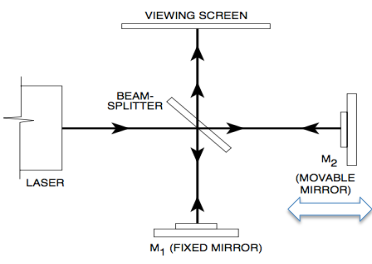
\includegraphics[width=0.5\textwidth]{michelson-interferometer/michelson-schematic.png}
	\caption{Schematic of a Michelson interferometer.}\label{mi:fig:schematic}
\end{figure}

In this way the original beam of light splits, and portions of the resulting beams are brought back together. The
beams are from the same source and their phases are hence highly correlated. When mirror $M_2$ is moved (closer to or
further from the laser source) the \textit{difference} in the path length of the light beams $(B$M$_1 - B$M$_2)$ changes, resulting in
changed in interference fringes. For a clear visualization of the effect, a lens placed between the laser source and the
beam-splitter spreads out the beam. An interference pattern of dark and bright rings, or \textit{fringes}, is seen on the
viewing screen. The rings are generated by interference of different portions of the laser beam, expanded to easy
visibility by the lens.

\section{Setup and Alignment of the interferometer}

Before you do an experiment with the interferometer, you'll need to ensure that it is aligned and an interference pattern (a set of concentric alternating light and dark rings) is clearly seen on the viewing screen when the laser is turned on. If that's true, then you can skip ahead to the next section.

Our laboratory setup is shown in Figure~\ref{mi:fig:setup-photo}.

\begin{framed}
	\textbf{Warning: Laser Hazard!} Lasers can cause temporary and permanent damage to eyes when exposed directly or through reflective surfaces.
	
	The following rules reduce the risk of eye exposure to laser light:
	\begin{enumerate}
		\item Do not direct the laser beam into anyone's eye.
		\item Be aware of the laser reflecting off of mirror-like surfaces and where that beam goes.
		\item Turn off the laser when not in use.
		\item Keep the laser pointing horizontally and near the plane of the table, while keep your eyes above that plane.
		\item To determine whether the laser is on, put your hand or a light-colored object in front of the beam, rather than looking into the laser aperture.
	\end{enumerate}
\end{framed}

\begin{figure}
	\centering
	\includegraphics[width=\textwidth]{michelson-interferometer/setup-photo.png}
	\caption{Our particular classroom setup, fully assembled and aligned, showing an interference pattern on the viewing screen.}\label{mi:fig:setup-photo}
\end{figure}

\begin{enumerate}
	\item The interferometer itself (this is part that has the optics) should be bolted to an optical rail at one end, with the
beamsplitter mirror facing the long end of the rail. Do so, if this isn't already in place.

	\item An aluminum block, with upward
facing magnets, should also be bolted into the rail near the other end.

	\item A steel plate, with an upturned edge, should
also be bolted to the rail, with the flat edge tight against edge of the interferometer.

	\item A 3⁄4” thick steel block, with two V-shaped grooves (one large and one small) should be placed on top of the aluminum block with magnets, with the V-shaped grooves facing upward; the magnets will keep the steel block in place.
	
	\item To begin, orient the block so the V-shaped grooves are aligned with the long axis of the rail, and the larger groove is toward the side of the rail opposite from the position of M$_1$ in the interferometer. The grooves are mount points for lasers, of two different barrel widths.
	
	\item Place a laser in one of the V-shaped grooves, pointed toward the interferometer, and turn it on. If necessary, you may secure the laser to the block using an elastic band or similar, taking advantage of the small grooves on the underside of the block that allow easy passage of a securing band.
	
	\item Place a viewing screen so that it is opposite M$_1$, or use a convenient light-colored wall.
	
	\item Loosen the thumbscrew that holds the beam-splitter and rotate the beam-splitter so it is out of the beam path of the
	laser as shown in Figure~\ref{mi:fig:adjusting-m1}.
	
	\begin{figure}
		\centering
		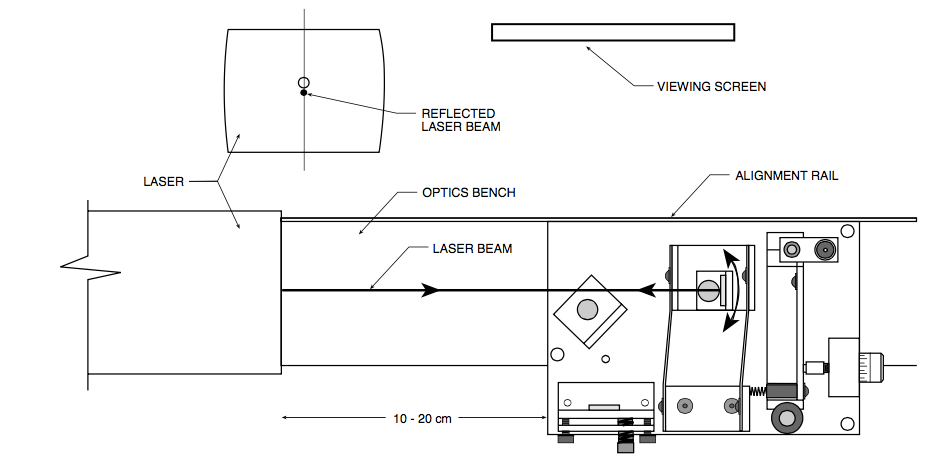
\includegraphics[width=\textwidth]{michelson-interferometer/adjusting-m1.png}
		\caption{Adjusting the M$_1$ mirror.}\label{mi:fig:adjusting-m1}
	\end{figure}
	
	\item Align the steel block holding the laser so that the beam hits M$_2$ as well-centered as
	possible; you can slide the steel block, rotate it (the magnets hold it in place but allow freedom of movement), and place paper in the groove under the laser to adjust the height or angle.
	Your goal should be to have the laser beam parallel to the long axis of the optical rail, and centered on M$_2$.
	
	\item The reflected beam should return back to the laser head. (The reflected beam need not be --- and likely won’t be --- at the
	same height as the incident beam, but it should return along the same path when viewed from exactly above. Hold
	your hand or piece of paper near the laser head --- without blocking the outgoing beam --- to see where the return beam
	is going.) If the return beam is not going where you want, you may loosen the thumbscrew that holds M$_2$ and adjust
	the rotation of M$_2$ so the laser beam is reflected directly back toward the laser head. Once satisfied with the alignment,
	hold M$_2$ in position and tighten the thumbscrew.
	
	\item Adjust the alignment screws on the mount for the mirror M$_2$, so that the mount plate does not appear tilted (see Figure~\ref{mi:fig:aligning-spots} for the location of these screws). When viewed from above there is gap between the plate holding the mirror and a
	second plate behind it. Adjust the screws so the plates appear parallel.
	
	\begin{figure}
		\centering
		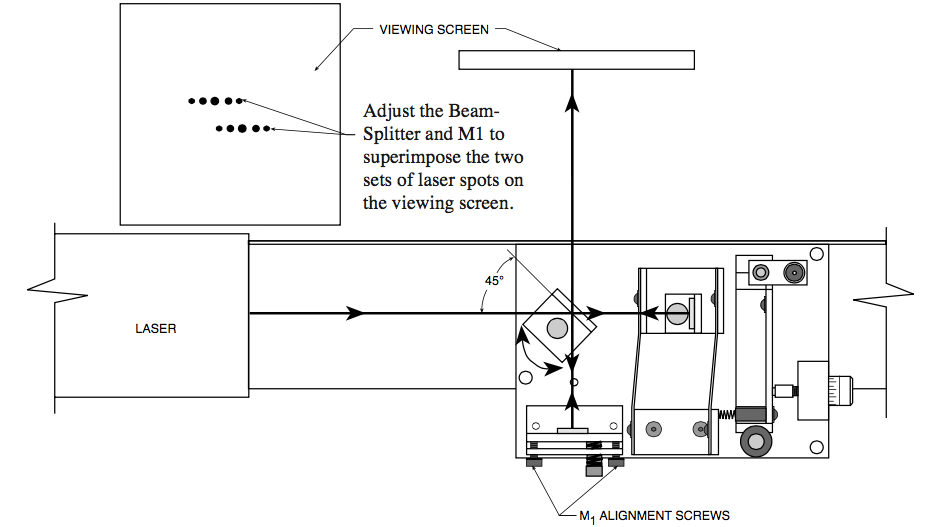
\includegraphics[width=\textwidth]{michelson-interferometer/aligning-laser-spots.png}
		\caption{Aligning the laser spots.}\label{mi:fig:aligning-spots}
	\end{figure}

	\item Rotate the beam-splitter so its surface is at an angle approximately 45 with the incident beam from the laser (see Figure~\ref{mi:fig:aligning-spots}). You will see two sets of laser spots on the viewing screen, corresponding to the two paths that the beam takes in reaching the screen. (Each path results in more than one laser spot because of multiple reflections within the beam-
	splitter.) Adjust the beam-splitter so the two sets of laser spots are as close as possible, then tighten the thumbscrew
	to secure the beam-splitter.
	
	\item Now, using the alignment screws, adjust the angle of M$_1$ until the two sets of laser spots are superimposed on the
	viewing screen (the two brightest spots must be superimposed).
	
	\item Place the 18 mm focal length lens on the optical bench on the steel plate between the laser mount and the
	interferometer (see Figure~\ref{mi:fig:positioning-lens} for setup and resulting desired pattern). The lens is in a holder that is magnetically coupled to a base; align one long edge of the base along the
	upturned edge of the steel plate. The lens should be about 10cm from the beamsplitter. Adjust the position of the lens
	on the holder so the light from the laser, now spread out by the lens, strikes the center of the beam-splitter. Move the
	lens vertically by sliding the lens holder vertically against the base (the magnets again allow freedom of movement
	here. The simplest way to move lens horizontally is to just slide the base lone the edge of the steel plate below. You
	should see an illuminated oval (or at least a partially illuminated oval) of laser light on the viewing screen. Adjust the
	lens position until the oval is as uniformly illuminated as you can achieve. Now, if you have performed the alignment
	correctly, you will see not just an illuminated oval, but a interference pattern of concentric rings on the viewing screen.
	If the alignment is not just right, the center of the fringe pattern may not be visible on the screen. Adjust the alignment
	screws on M$_1$ very slowly as needed to center the pattern. \textit{NOTE: aligning the interferometer so that you get fringes
	can be fiddly...if necessary, try a few times, and seek help from your TA if you cannot make it work.}

	\begin{figure}
		\centering
		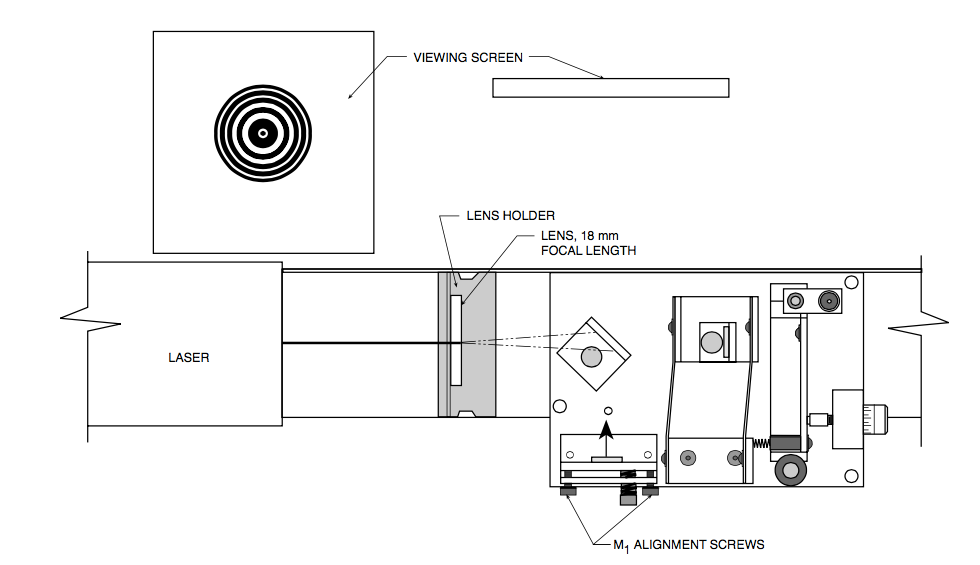
\includegraphics[width=\textwidth]{michelson-interferometer/positioning-lens.png}
		\caption{Positioning the lens, and fine alignment of M$_1$.}\label{mi:fig:positioning-lens}
	\end{figure}

\end{enumerate}

\section{Relating wavelength to distance changes}

By moving the mirror M$_2$, the path length of one of the beams can be varied. Since the beam traverses the path
between M$_2$ and the beam-splitter twice, moving M$_2$ 1/4 wavelength nearer to the beam-splitter will reduce the optical
path of that beam by 1/2 wavelength. The interference pattern will change; the radii of the maxima will be reduced so
they now occupy the position of the former minima. If M$_2$ is moved an additional 1/4 wavelength closer to the beam-splitter, the radii of the maxima will again be reduced so maxima and minima trade positions. However, this new
arrangement will be indistinguishable from the original pattern. So when moving the position of M$_2$, you will observe the
fringes ``moving'' reproducing the original pattern.

The movement distance $d$ of the mirror M$_2$ and the corresponding number of times $m$ the fringe pattern is restored to its original state are related by
\begin{equation}\label{mi:eq:interference}
 m \lambda = 2 d \, ,
\end{equation}
where $\lambda$ is the wavelength of the incident light. Thus, very small displacements d can be measured by counting the number m. Conversely, the wavelength of the light
can be accurately determined if d is known. In your interferometer, a knob with a micrometer scale can be used to move
M$_2$. M$_2$ is help on a lever spring arm that is anchored to the baseplate of the interferometer at another location. The
micrometer knob pushes on another arm that applies tension to a strap that is coupled to the lever arm holding M$_2$.

\section{Experiment 1: determining the wavelength of the laser}

\textbf{Goal:} Determine the wavelength of a laser.

\textbf{Rubric rows to be assessed:} D1, D4, F1, F2, G2, G4, G5.

\textbf{Available equipment:} Michelson interferometer mounted on optical rail, laser

Since this is such a sensitive measurement, we provide a measurement procedure for you. In order to determine the wavelength, you'll measure the number of fringes moved and the distance the mirror moved  and use Equation~\ref{mi:eq:interference} to calculate the wavelength of the laser.

\subsection{Procedure}

\begin{enumerate}
	\item\label{mi:step:micro} Adjust the micrometer knob so the lever arm is approximately parallel with the short edge of the interferometer
	baseplate. In this position the relationship between knob rotation and mirror movement is most nearly linear.
	
	\item Turn the micrometer knob one full turn counterclockwise. Continue turning counterclockwise until the zero on the
	knob is aligned with the index mark. \textit{(NOTE: Whenever you reverse the direction in which you turn the micrometer
	knob, there is a small amount of give before the mirror begins to move. This is called mechanical backlash, and is
	present in any mechanical system involving reversals in direction of movement. By beginning with a full
	counterclockwise turn, and then turning only counterclockwise when counting fringes, you can eliminate backlash
	in your measurement.)}

	\item Place a sheet of paper on the viewing screen, secure it with tape, and make a reference mark on the paper between
	two of the fringes. This will help you in keeping count of the fringes.
	
	\item Now turn counterclockwise the knob until you have counted about 40 movements of the fringes.
	
	\item\label{mi:step:record} Record the measurement on the knob as distance $d$ and record the number of fringe movements $m$.
	
	\item Repeat Steps~\ref{mi:step:micro}--\ref{mi:step:record} 2 more times, for a total of 3 measurements.
\end{enumerate}

Use your findings to determine the wavelength of the laser, including an estimate of the uncertainty in your reported value. Include the following in your report:
\begin{enumerate}
	\item A statement of the problem you are solving (D1).
	
	\item A clear, concise description of the experimental setup and procedure (F1).
	
	\item A table of the data that you took (G4).
	
	\item A description of your analysis that led you to find the wavelength (G5).
	
	\item A description, with calculations shown, of your determination of the uncertainty in the wavelength (G2).
	
	\item A final judgment of what your team thinks the wavelength of the laser is, based on your experimental results, including uncertainty (D4).
	
	\item A discussion of the findings of the experiment and why it's helpful (for you and/or for science) (F2).
\end{enumerate}

\section{Experiment 2: Measuring distance changes}

In your individual homework, you will determine distance changes in one of the arms of the interferometer, not caused by gravitational waves, like in LIGO, but by thermal expansion and the slight bending of the baseplate of the apparatus. During lab, take the following data, both without turning the knob to move the mirror:

\begin{enumerate}
	\item The clear strap that pulls the mirror back and forth will expand and contract with heating and cooling (like most solids). Measure the number of fringe movements that happen when you hold your finger very close to the strap, within a few millimeters, for 20--30 seconds.
	
	\item The baseplate is very sturdy, yet still bends when uneven pressure is applied, even if imperceptible to our senses. Measure the number of fringe movements that happen when you press lightly on the baseplate between one of the mirrors and the beam-splitter.
\end{enumerate}

\section{Individual homework}

\begin{enumerate}
	\item Use the data taken during Experiment 2 to determine the path length changes in each case (include calculation of uncertainty).
	
	\item Report on if this is surprising to you or not, either that the distance change is as large or small as it is, or the fact that you can measure such a small distance change.
	
	\item For what useful or fun purpose could this kind of sensitive measurement technique be used?
\end{enumerate}

\chapter{Black hole at the Galactic center? (stellar orbits)}

%TODO replace homework with actually doable and physical arguments
%TODO restructure lab to make sense, be clear, organized
%TODO make equal-area section length^2, not arcsec^2

\section{``Observing'' Black Holes}

Black Holes are robustly predicted by Einstein's theory of General Relativity, the current state-of-
the-art in mathematical explanations of gravitational phenomenon. It has also been demonstrated
theoretically that such extreme objects naturally arise in the late-stages of stellar evolution for the
most massive stars. However, they are difficult to observe for a simple reason: by their very nature (as
suggested by their name), they do not emit light. Nonetheless, their presence can be inferred indirectly
through their gravitational effect on other objects. Astronomers and physicists have discovered so many
independent and corroborating lines of evidence of this type detected that the existence of black holes
is now considered a well-established scientific fact.

The detection of gravitational waves by the Laser Interferometer Gravitational-Wave Observatory
(LIGO) in 2017 is arguably the most stunning and conclusive evidence of this to date. In a
beautiful demonstration of the validity of General Relativity, the perturbations in space and time
(Gravitational Waves) characteristically generated by the coalescence of a binary black hole pair were
detected on Earth after having traveled at the speed of light from their source roughly one billion light
years away. The clarity of this signal and its agreement with predictions have all but conclusively
determined the existence of black holes.

However, less direct (but nonetheless extremely convincing) evidence for the existence of black holes
had been well known in observational astronomy for some time. In this lab, you will explore one of the
most striking examples of these observational signatures: the orbits of stars around Sag A*, the radio source that is collocated with the `dark attractor' at the center of our galaxy that is almost certainly a Super-Massive Black Hole (SMBH). Astronomers now know that almost all galaxies have such behemoths at their centers, and that they likely play a fundamental role in galaxy evolution. The discovery of one at the center of the Milky Way (roughly 8 kpc distant) was an important step in the development of this SMBH paradigm. In this lab, you will partially reproduce a simplified version of the analysis that led astronomers to this exciting conclusion.

\textbf{Rubric Rows to be assessed:} C4 and C5 (for Kepler's 2nd Law); D8, D9, and G1 (for Kepler's 3rd Law mass estimation); F1 and F2 (for all parts)

\section{Newtonian Dynamics and Orbital Dynamics Basics}

The trajectories of objects moving under the influence of gravity are generally called \textit{orbits}. Newton's
Law of Gravity, while not an adequate description for extreme gravitational fields, is nonetheless a good
approximation generally and in the specific cases of orbits we'll be examining. It is given by
\begin{equation}\label{gc:eq:newton}
 F_\textrm{grav} = G \frac{m_1 \: m_2}{r^2} \, ,
\end{equation}
where $F_\textrm{grav}$ is the force of gravity between any two objects of mass $m_1$ and $m_2$ a distance $r$ from each other. $G$ is Newton's Gravitational Constant, whose value in CGS (Centimeters Grams Seconds) units
is $6.67 \times 10^{-8}\:\textrm{cm}^3 \: \textrm{g}^{-1} \: \textrm{s}^{-2}$. The gravitational force is attractive: it pulls objects together. This, coupled
with Newton's Second Law of Motion relating the force acted upon an object $F$ and its acceleration $a$,
\begin{equation}
 F = ma \,,
\end{equation}
tells us that \textit{the acceleration of an object due to gravity will be greater in stronger gravitational fields}.
These two fundamental physical laws can be used to derive the properties of Newtonian gravitational
orbital motion. We won't do so here, but instead just cover some of the key implications, concisely
stated by Kepler's Laws of Orbital Motion. These Laws, which are concise mathematical descriptions
of how the planets move in the Solar System, preceded Newton's work by nearly a century, and were
based solely on observational data. Newton's work on gravity and motion explained, at a deeper level,
why Kepler's Laws are as they are.

\subsection{Kepler's Laws}

\subsubsection{Kepler's First Law}

Kepler’s First Law states that \textbf{A planet orbits the Sun in an ellipse, with the Sun at one focus
of the ellipse.} This is true generally for any mass orbiting a much more massive object. An \textit{ellipse} is a
generalization of a circle, allowing for the circle to be stretched along a certain direction. See Figure~\ref{gc:fig:ellipse} for details.

\begin{figure}
	\centering
	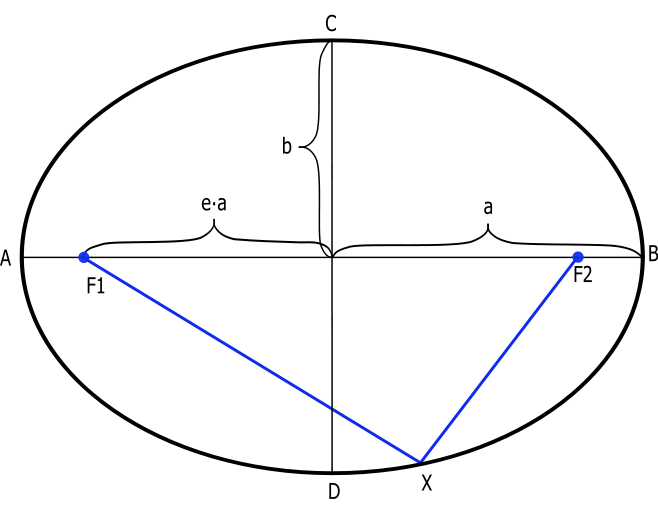
\includegraphics[width=0.6\textwidth]{galactic-center/ellipse.png}
	\caption{The geometry of an ellipse: $a$ is the semi-major axis of the ellipse, F1 and F2 are each a
		focus of the ellipse, $b$ is the semi-minor axis, and $e$ is the eccentricity. The eccentricity describes
		the extent to which the ellipse is oblong: an ellipse with $e = 0$ is just a circle. The foci are defined such
		that the distance from F1 to X, added to the distance from F2 to X, is the same no matter where X
		is located on the ellipse. For a circle, the foci coincide at the center. The Newtonian generalization of
		Kepler's First Law tells us that a small mass will orbit a much larger mass on an ellipse, and the larger
		mass will be located at one of the foci.}\label{gc:fig:ellipse}
\end{figure}

\subsubsection{Kepler's Second Law}

The second law states that \textbf{a line connecting a planet to the Sun sweeps out equal areas in
equal time intervals}. This concept is demonstrated in Figure~\ref{gc:fig:keplers-2nd-ellipse}. As a consequence of this, when a
planet is closer to the sun, it orbits with a faster velocity. Furthermore, planets that have more circular
orbits will have more uniform velocities over the course of their orbit than those with very eccentric
orbits.

\begin{figure}
	\centering
	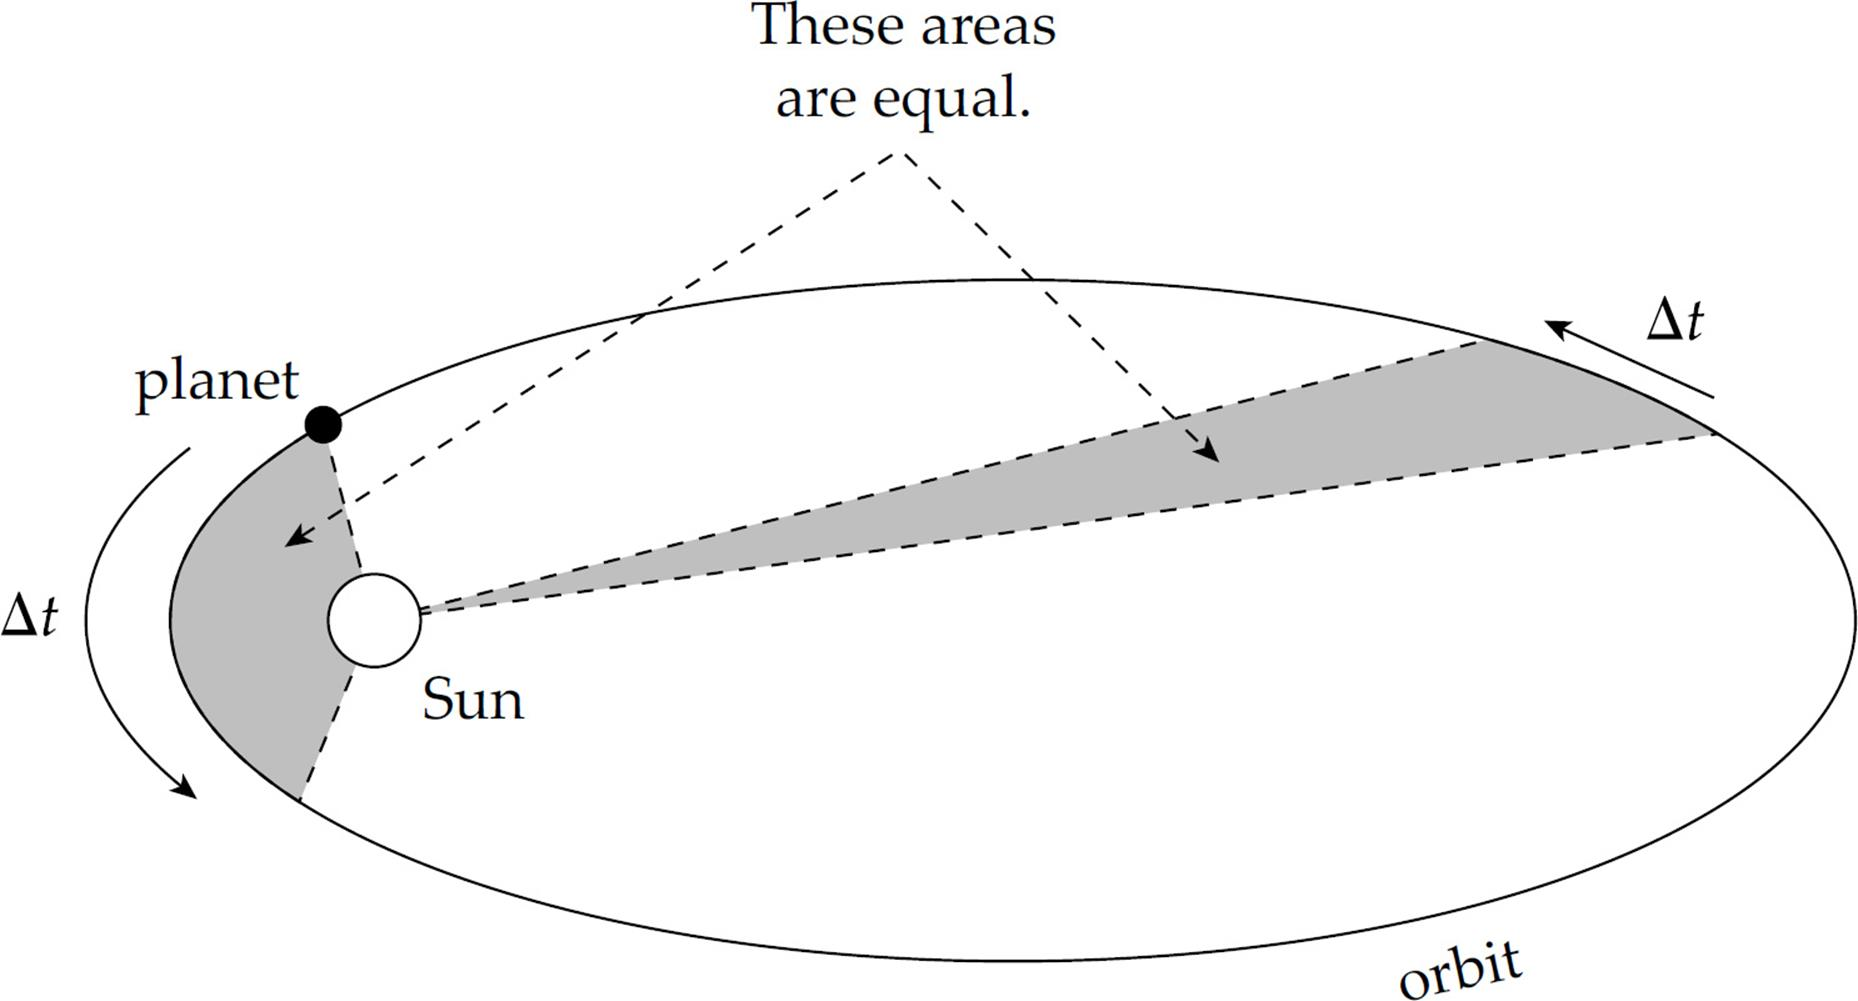
\includegraphics[width=0.7\textwidth]{galactic-center/keplers-2nd-ellipse.png}
	\caption{Illustration of Kepler’s Second Law. The shaded regions are of equal area, so by Kepler’s Second Law, the
		planet passes through each region of the orbit in the same amount of time. Since the region of the orbit
		where the planet is closest to the Sun is a much further distance, and speed is change in position over
		change in time, the planet will move with a much faster average speed than at the other portion of the
		orbit, far away from the sun.}\label{gc:fig:keplers-2nd-ellipse}
\end{figure}

\subsubsection{Kepler's Third Law}

Kepler’s Third law addresses the path of an object $m$ as it orbits a much more massive object of mass $M$. Specifically, it relates the orbital period $P$ (the time it takes for one complete orbit to occur) to the semi-major axis $a$ of the ellipse according to
\begin{equation}\label{gc:eq:kepler-3}
 P^2 = \frac{4 \pi^2}{G M} a^3 \,,
\end{equation}
where other objects are also considered to be not affecting the orbit of $m$. \textbf{This is the
	equation you will be using in the central calculation of the lab.}

An important qualification to be made about Kepler’s Laws is that they apply only to two-body
systems. Kepler’s Third law breaks down when you have more than 2 orbiting objects in a system.
However, they are nonetheless a very good approximation for the orbits of small masses around a much
larger mass, in which case the gravitational force of the massive object dominates over the intra-small-
object interactions, and thus each smaller body approximately behaves independently from the other
small objects. And so the motion of each small object, to a good approximation, can be modeled by
Kepler’s Laws.

\subsection{Escape speed}

Another important concept in orbital dynamics --- which comes from the general Newtonian understanding of orbits --- is that of the escape speed. This is the minimum speed that an object must reach
to break out of its orbit at a certain radius from the central massive object. The escape speed $v_\textrm{escape}$ at a
distance $r$ from the center of a mass $M$ is given by
\begin{equation}\label{gc:eq:escape-speed}
 v_\textrm{escape} = \sqrt{\frac{2 G M}{r}} \,.
\end{equation}
An orbiting object that achieves a speed greater than this is unbound to the object it is orbiting, and will escape its gravitational pull, flying out of the system entirely.

\section{General Relativity}

Despite the great success of Newtonian dynamics in explaining a wide variety of the celestial motions
that we observe, this picture of gravity is incomplete and inaccurate in the most extreme regimes,
where General Relativity is required. A fully self-consistent description of relativity is well beyond the
scope of these notes (or this course), but the fundamental conceptual premise is easily stated: gravity
is not a magical “attraction at a distance” between objects with mass, but rather the result of curved
space-time, which is an effect of all mass. A helpful analogy is that of a sheet of fabric being depressed
by a massive object (see Figure~\ref{gc:fig:gen-rel-sheet}). Other objects placed on this depressed fabric will begin orbiting
around the massive object.

\begin{figure}
	\centering
	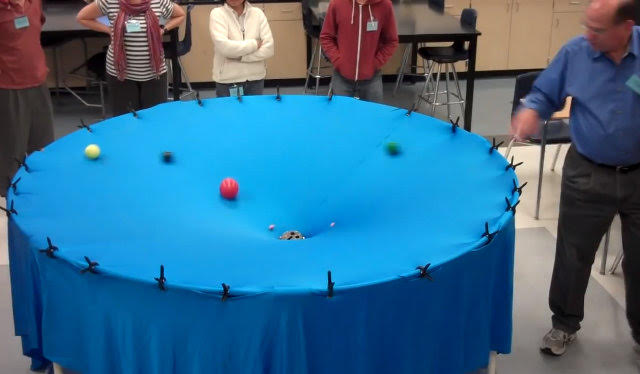
\includegraphics[width=\textwidth]{galactic-center/gen-rel-sheet.png}
	\caption{General Relativity Analogy.}\label{gc:fig:gen-rel-sheet}
\end{figure}

For the purpose of this lab, the most important consequence of this paradigm shift is the fact that
gravity thus affects everything, including even massless objects like light, in exactly the same way that
it does massive objects, since they also travel through space-time. Thus, there might exist objects with 
such extremely strong gravitational fields (and thus extremely contorted spacetimes) that even light
cannot escape. Since Special Relativity (Einstein’s original theory of relativity, which he later built
off of to develop General Relativity) tells us that light sets the cosmic speed limit, nothing else can
escape either. These are termed Black Holes. We should note that, while we are assessing observational
evidence for a black-hole in this lab, we will nonetheless use the Newtonian gravitational framework to
understand our observations, sine the gravitational fields experienced by the stars we are observing are
--- to an excellent approximation --- well-described by Newtonian gravity.

\section{Schwarzschild Radii}

One can extend Newtonian dynamical arguments to estimate the relevant scales for relativistic objects.
For example, in the context of Newtonian Gravitation, one can think of a Black Hole as an object that
has an escape velocity greater than the speed of light. Thus one can substitute the speed of light into
the equation for the escape speed (Equation~\ref{gc:eq:escape-speed}) to estimate the radius of a Black Hole,
\begin{equation}
 R_\textrm{Schwarzschild} = \frac{2 G M}{c^2} \,
\end{equation}
where $c = 2.998 \times 10^{10}\:\mathrm{cm}/\mathrm{s}$ is the speed of light. $R_\textrm{Schwarzschild}$ is called the Schwarzschild Radius, and is actually the correct value predicted by General
Relativity for a certain class of black holes, so it’s a very good estimate. Any object dense enough to be
contained inside of its Schwarzschild radius must be a black hole.

\section{Lab Tasks}

For each of the following objects, a) calculate the Schwarzschild radius for that object’s mass, b) list
an everyday object of comparable size and c) find the ratio of the Schwarzschild to physical radius of
the object: (hint: do this in excel so you don’t have to repeat the calculation \textit{ad nauseum})
\begin{enumerate}
	\item One of your group members.
	\item the Earth.
	\item the Sun.
	\item the Solar System.
	\item The Milky Way Galaxy.
\end{enumerate}

\section{Orbit Simulator and 3D model}

First we will explore some interactive animations of orbital motion, then a three-dimensional rendering
of the real scientific data that we will analyze in the second part of this lab.

\section{Lab Tasks}
\begin{enumerate}
	\item Go to
	
	\url{https://www.windows2universe.org/physical_science/physics/mechanics/orbit/orbit_shape_interactive.html}. This website allows one to adjust the shape of an orbit for a hypothetical planet in the solar system.

	\begin{enumerate}
		\item Set the semi-major axis at 1AU (the radius of Earth’s nearly-circular orbit), and the eccentricity to it’s maximum value (0.9). By observing the motion of the planet with respect to
		Earth, verify (qualitatively, no need for numerical calculations here) each of Kepler’s Three
		Laws.
		
		\item Based on the orbital dynamics your observe, what simplifying approximations can you tell
		are being made in the calculation that goes into this animation? Particularly notice when
		your test planet comes close to another planet in its orbit. Do their orbits remain the same?
		Should they?
	\end{enumerate}

	\item Now go to \url{www.astro.ucla.edu/~ghezgroup/gc/animations.html}, the website for the UCLA
	Galactic Center Group, where you will find a number of informative graphics that relate to the
	content of this lab. On the bottom-right under the section “3D Movie of Stellar Orbits in the Central Parsec” is a volume-rendered video of stars orbiting Sag A* --- the radio and X-
	ray source at the center of the galaxy, the mass of which you will be measuring in the next
	section.
	
	\item Expand the video to full-screen and pay attention to one or two of the stellar orbits,
	which are show in full by the video. Pause the video at several points during the video. How
	do the 2D shapes of the orbits on the image change as the camera angle moves? How does the
	inclination of the orbital plane in our field-of-view modify the observed orbital shape? How might
	this confuse the determination of orbital parameters? How can we disentangle this? (hint: think
	about Kepler’s Laws and the location of the foci). What kind of errors in our measurement will
	result from an assumption that we are looking at an orbit directly from above? Will this cause the inferred mass to be over- or under-estimated? (See Scientific Ability Rubric Row D9 in Table~\ref{rubric:d}).
	
	\item As well, consider the spatial orientation of the orbits here with reference to those of the solar
	system, considered in the previous task. Is there any coherent organization of stellar orbits
	around the black hole in this video? How does this compare to the orientation of planets in
	the solar system? What might be a physical reason for this difference (hint: think about their
	respective formation mechanisms).
\end{enumerate}

\section{Sag A* Mass Estimation}

Now you will roughly measure the mass of Sag A* by extracting the positions of several stars orbiting
the galactic center from a published YouTube video that illustrates the stellar dynamics observed by
the UCLA Galactic Center research group. Their data comes from the largest research telescopes on
the planet, observing the Galactic Center using sophisticated imaging cameras that give images even
sharper than those produced by the Hubble Space Telescope. We will ”observe” the video of their
measurements, to illustrate the process of data → measurement → analysis → conclusion (a mass!).

\subsection{Lab Tasks}

\begin{enumerate}
	\item Go to \url{https://www.youtube.com/watch?v=7vcSKbXnLJA}. This movie shows observations of Sag
	A* and the surrounding stellar cluster taken over more than a decade. Watch the video, and record
	your impressions in light of your previous activities on orbital dynamics and the introductory
	information. What is going on here? How might this be used as evidence for the existence
	of a SMBH at the galactic center? What other corroborating data would you want/need to
	substantiate that claim?
	
	\item After watching several times and recording your initial impressions, you will now take some crude “measurements” of the data in the video. You will then use these to both verify Kepler’s Second Law and make an order-of-magnitude estimate of Sag A*’s mass using Kepler’s Third Law.
	
	Data acquisition:
	\begin{enumerate}
		\item Restart the video and take a screen-grab of the first frame using the PrintScreen function (you will
		be doing this several times so make a folder in which to save your screenshots).
		
		\item Let the animation advance by one second (so that the stars have begun moving in their
		orbits), pause, and capture another screen image. Do this for each second of the animation,
		giving you 9 separate images of the stars in different positions on their orbits.
		
		\item For Kepler's Second Law, you will need to measure several areas traced out by an orbit in the same time duration. Open the first frame in the ImageJ software. Note the white arrow on the left of the
		screen indicating the angular scale of the image.
		%Notice that Kepler's law describes areas, while we are limited, at present, to angular areas, since we are not including how far away the stars are to us. This approximation should be just fine for testing the law, as long as the angle is small.
		
		\item On the menu tab click the straight line icon
		located at the 5th position to the left. Click one end of the arrow and drag the line from one
		end of the angular scale to the other. Now go to the Analyze dropdown menu and select Set
		Scale. Set the known distance to be the distance of the scale, 0.1 arcseconds. (Look up how
		to convert from arcseconds to degrees, and then to radians).
		
		\item Once the scale is set, select the straight line icon again and drag the line from the star symbol
		(representing Sag A*) to the orbiting star you want to measure. The measure hotkey is ”m.”
		This will now give you the angular distance from Sag A* to the orbiting star in arcseconds.
		It will also give you an angle value that will allow you to measure the angular rotation of
		the star in its orbit. Record these values for both S0-2 and S0-37 in the first 2 columns of a data table set up like Table~\ref{gc:tab:orbits}, one table for each of these stars, one row for every frame you captured.
		
\begin{table}
	\centering
	\begin{tabular}{c|c|c|c|c|c}
		frame & $d$ (arcseconds) & $s$ (cm) & $\theta$ (radians) & $\Delta \theta$ (radians) & $A$ (cm$^2$)
		\\ \midrule
		1 & & & & \cellcolor{black!25} & \cellcolor{black!25}
		\\ \midrule
		2 & & & & & 
		\\ \midrule
		3 & & & &  &
		\\ \midrule
		4 & & & &  &
		\\ \midrule
		5 & & & & &
		\\ \midrule
		6 & & & & &
		\\ \midrule
		7 & & & & &
		\\ \midrule
		8 & & & & &
		\\ \midrule
		9 & & & & &
		\\ \bottomrule
	\end{tabular}
	\caption{Data table for one stellar orbit. Note that you will not have any calculations for the gray cells for frame 1, since there is no previous frame to compare to.}\label{gc:tab:orbits}
\end{table}		

	\end{enumerate}

	\item Kepler's Laws:
	\begin{enumerate}
		\item Kepler's Second Law: This data can now be used to test Kepler’s Second Law. The area
		covered by a line connecting the planet and Sag A* between measurements $i$ and $i - 1$ can
		be given by
		\begin{equation}
		 A_i = \pi \left( \frac{s_{i} + s_{i-1}}{2} \right)^2 \left( \frac{\theta_{i}-\theta_{i-1}}{2\pi} \right) \,,
		\end{equation}
		which approximates the swept area as the sector of a circle. To compute the distances $s_i$ from the angular distances $d_i$, convert $d$ to radians and multiply by the distance to Sag A*, $2.47 \pm 0.05 \times 10^{22}\:$cm.  Add this calculation for each
		segment and both stars to the data table. Does Kepler’s Second Law hold? Discuss any
		discrepancies and how you might account for them (Rubric Rows C4, C7, C8).
		
		\item Kepler’s Third Law: Now you will use Kepler’s Third Law, given in the introduction, to
		calculate the central mass around which these objects are orbiting. Go back to the final
		frame of the video and use the traced orbits to estimate the semi-major axis for both S0-2
		and S0-37. This estimated length is an angular length in arcseconds and should be converted to a physical length in centimeters. First convert the arcseconds to radians, then multiply it by the distance from Earth to Sag A*, and use the timestamps on
		the video to estimate the orbital periods in seconds. Note that, while this is straightforward for S0-2
		since it completes a full orbit in the span of the video, this is less obvious for S0-37. The
		key here is that S0-37 has a circular orbit. Use Kepler’s Laws and the previous discussion of
		oribital inclination observational effects to determine how S0-37’s period can be estimated
		from the given data. What approximations and assumptions need to be made to justify the
		use of this equation for the system we’re observing (Rubric Rows D8, D9)?
		
		\item Once you have done this calculation, compare your obtained value of M to the best-estimate
		mass of the central SMBH of $M_\mathrm{bh} = 4.0 \times 10^6\:\textrm{M}_\textrm{\astrosun}$ (Boehle \textit{et al.} 2016). How far off was your
		estimate? Was it within your estimated error (See Section~\ref{unc:sec:comparing})? List all possible sources of error and bias,
		both procedural and physical, in this calculation. Particularly, think about the applicability
		of Kepler’s Third Law to the physical system we are measuring (Rubric Rows G1, G2).
	\end{enumerate}

	\item Sag A* Size estimation
	\begin{enumerate}
		\item Now, that we have a mass estimate for Sag A*, the next step is to place upper limits on
		its physical size. Using the last frame in the video, try to use the paths of the orbits that
		come closest to the star symbol indicating Sag A* to place an upper limit on its radius. To
		determine that Sag A* is a black hole, we need to make an estimate of its physical extent,
		which will allow us to rule out all other plausible forms of matter (at least as far as we know).
		What is the physical value of this upper limit? Given the mass you calculated, how does
		this compare to its Schwarzschild radius?
		
		\item While this suggests that the central attractor is an extremely dense object, we can place
		even tighter constraints on its physical extent based on the timescales of its fluctuations
		in electromagnetic observation. Sag A* is lacking in any prominent optical emission, it is
		nonetheless observable in radio and X-ray frequencies. As well, we observe it’s brightness in
		these frequencies to flare (Figure~\ref{gc:fig:light-curve}) somewhat regularly on the order of once per day, with
		actual flare events lasting much less time. Since the speed of light is finite, when an object
		flares, light from the side of the object opposite the observer will become visible later than
		that from the side closest to the observer. Thus, the time it takes for the object to flare
		will be limited by light-travel time across the object. This allows us to use the light-travel
		distance over the timescale of the flare as an upper-limit on the physical extent of the object.
		Use Figure~\ref{gc:fig:light-curve} to do just this. Calculate the corresponding angular size of this distance as
		observed from earth (in arcseconds, for easy comparison with the video data). How does this
		measure compare with Schwarzschild radius of a black hole of the mass you measured?
		
		\begin{figure}
			\centering
			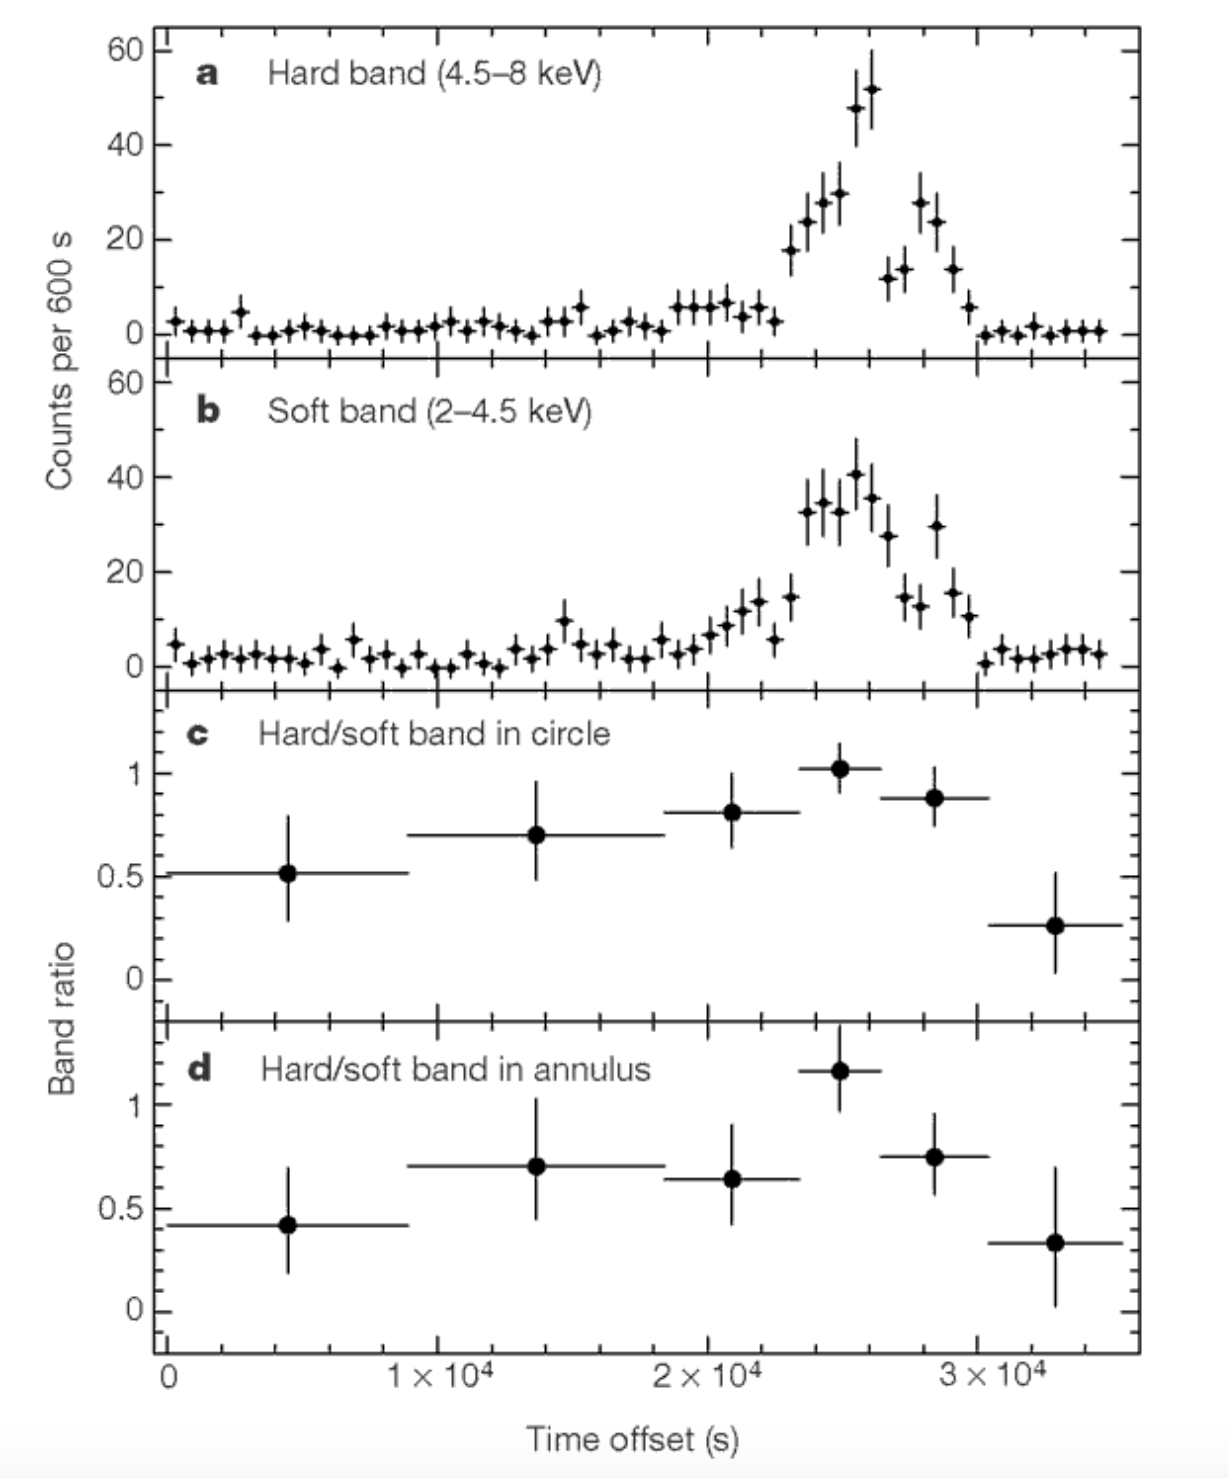
\includegraphics[width=0.7\textwidth]{galactic-center/sag-a-light-curve.png}
			\caption{Sag A* light curve, showing significant flaring on the timescale of a day.
				(from \url{https://heasarc.gsfc.nasa.gov/docs/objects/galaxies/sag-a star.html})}\label{gc:fig:light-curve}
		\end{figure}
	\end{enumerate}
\end{enumerate}

\section{Individual Homework}

There is no individual homework for this lab.

%Now that we have determined that Sag A* is an extremely dense, massive object --- but not quite certainly a black hole --- we are left to make plausibility arguments that allow us to
%eliminate all other possible forms of matter. For each category of astrophysical objects listed
%below, estimate the observational signatures of a hypothetical object with the mass you’ve
%measured for Sag A*. Decide whether or not the estimated observable properties can be used
%to rule out this alternative to a black hole.
%\begin{enumerate}
%	\item Main-Sequence Star/Cluster (Hint: the luminosity of massive stars scales as $M^4$, so
%	what luminosity would a Sag A*-star have? What would be the luminosity of a cluster
%	of sun-like stars with a total mass equal to that of Sag A*?)
%	
%	\item Brown Dwarf Star Cluster (Hint: A typical brown dwarf luminosity is $\sim 10^{-4} L_\textrm{\astrosun}$ and
%	the maximum brown dwarf mass is $0.08M_\textrm{\astrosun}$. Brown dwarfs more massive than this are
%	just stars, which you presumably ruled out above.)
%	
%	\item White Dwarf Star Cluster (Hint: a typical White Dwarf luminosity is $0.03L_\textrm{\astrosun}$, and the
%	maximum white dwarf mass is $1.4M_\textrm{\astrosun}$. There are fundamental physical arguments that
%	preclude the stable existence of a white dwarf above this mass.)
%	
%	\item Neutron Star Star Cluster (Hint: a typical Neutron Star luminosity is $10^{-6} L_\textrm{\astrosun}$ , and the
%	maximum neutron star mass is estimated to be $1.4M_\textrm{\astrosun}$. This maximum mass is also
%	derived from fundamental physics considerations). Would such a configuration, even if
%	hypothetically possible, be physically reasonable?
%\end{enumerate}
%\chapter{Observing Falling Filters}

	\begin{quotation}
		\textit{The ability to observe without evaluating is the highest form of intelligence.} \sourceatright{Jiddu Krishnamurti}
	\end{quotation}

While Mr.\ Krishnamuri may be making a stretch with his superlative, it remains true that observing without evaluating is essential for the creation of knowledge.
In our lives, we have bias (conceptions, self-constructed mental models) that we use as our lens to view the world.
These models are based on how each of us were socialized and on our subsequent experience.
To learn and create new knowledge, we must develop skill in observation.
In this lab, we will direct you to make detailed, careful quantitative observations, describe the patterns you find with mathematics, and finally make some wild guesses (``hypotheses'') about a more universal principle that explains this pattern that one could use to make predictions.
Due to time and brain constraints, we will not, in this lab, test those hypotheses.

\section*{Learning Goals}

 \begin{itemize}

  \item Conduct an observation experiment, including collecting data, finding and describing a pattern quantitatively, including presentation of data graphically and formulating a quantitative hypothesis.

  \item Use measurement uncertainty to describe physical quantities meaningfully.
  
  \item Format a lab report in a helpful way.
 \end{itemize}

\section*{The Scientific Cycle\protect\footnote{adapted from \cite{etkina_college_2014}}}

Astrophysics is an experimental science. To answer questions, astrophysicists do not just think and dream in their offices but constantly engage in experimental investigations. Astrophysicists use special measuring devices to observe phenomena (natural and planned), describe their observations (carefully record them using words, numbers, graphs, etc.), find repeating features called patterns (for example, the distance traveled by a falling object is directly proportional to the square of the time of flight), and then try to explain these patterns. By doing this, astrophysicists describe and answer the questions of ``why'' or ``how'' the phenomena happened and then deduce quantitative rules called mathematical models that explain the phenomena.

However, a deduced explanation or a mathematical model is not automatically accepted as true. Every model needs to undergo careful testing. When astrophysicists test a model, they use the model to predict the outcomes of new experiments. As long as there is no experiment whose outcome is inconsistent with predictions made using the model, it is not disproved. However, a new experiment could be devised tomorrow whose outcome is not consistent with the prediction made using the model. The point is that there is no way to ``prove'' a model once and for all. At best, the model just hasn't been disproven yet.

A simple example will help you understand some processes that physicists follow when they study the world. One model for the scientific process will also be described (there are other helpful models, and there is no one true ``scientific method''). Imagine that you walk into the house of your acquaintance Bob and see 10 tennis rackets of different quality and sizes. This is an \textbf{observational experiment}. During an observational experiment, a scientist collects data that seem important. Sometimes it is an accidental or unplanned experiment. The scientist has no prior expectation of the outcome. In this case, the number of tennis rackets and their quality and sizes represent the data. Having so many tennis rackets seems unusual to you, so you try to explain the data you collected (or, in other words, to explain why Bob has so many rackets) by devising several hypotheses. A \textbf{hypothesis} is an explanation that usually is based on some mechanism that is behind what is going on, or it can be a mathematical model describing the phenomenon. One hypothesis is that Bob has lots of children and they all play tennis. A second hypothesis is that Bob makes his living by fixing tennis rackets. A third hypothesis is that he is a thief who steals tennis rackets.

How do you decide which hypothesis is correct? You may reason: if Bob has many children who play tennis, and I walk around the house checking the sizes of clothes that I find, then I will find clothes of different sizes. Checking the clothing sizes is a new experiment, called a \textbf{testing experiment}. A testing experiment is different from an observational experiment. In a testing experiment, a specific hypothesis is being ``put on trial.'' This hypothesis is used to construct a clear expectation of the outcome of the experiment. This clear expectation (based on the hypothesis being tested) is called a \textbf{prediction}. So you conduct the testing experiment by walking around the house checking the closets. You do find clothes of different sizes. This is the \textbf{outcome} of your testing experiment. Does it mean for absolute certain that Bob has the rackets because all of his children play tennis? No; he could still be a racket repairman or a thief. Therefore, if the outcome of the testing experiment matches the prediction based on your hypothesis, you cannot say that you proved the hypothesis. All you can say is that you failed to disprove it. However, if you walk around the house and do not find any children's clothes, you can say with more confidence that the number of rackets in the house is not due to Bob having lots of children who play tennis. Still, this conclusion would only be valid if you made an \textbf{assumption}: Bob's children live in the house and wear clothes of different sizes. Generally, in order to reject a hypothesis, you need to check the additional assumptions you made and determine if they are reasonable.

Imagine you have rejected the first hypothesis (you didn't find any children's clothes). Next, you wish to test the hypothesis that Bob is a thief. This is your reasoning: \textit{If} Bob is a thief (the hypothesis), \textit{and} I walk around the house checking every drawer (the testing experiment), \textit{then} I will not find any receipts for the tennis rackets (the prediction). You perform the experiment and you find no receipts. Does it mean that Bob is a thief? He might just be a disorganized father of many children or a busy repairperson. However, if you find all the receipts, you can say with more confidence that he is not a thief (but he could still be a repairperson). Thus it is possible to disprove (rule out) a hypothesis, but it is not possible to prove it once and for all. The process that you went through to create and test your hypothesis is depicted in Figure~\ref{me:fig:isle}. At the end of your investigation you might be left with a hypothesis that you failed to disprove. As an astrophysicist you would now have some confidence in this hypothesis and start using it for practical applications, or \textbf{application experiments}.

\begin{figure}
	\centering
	\includegraphics[width=0.7\textwidth]{measurement/islegraphic.png}
	\caption{A model of the process some scientists go through to create knowledge.\cite{etkina_millikan_2015}}\label{me:fig:isle}
\end{figure}

\section*{Observation experiment: Observing falling filters}

In today's lab, you will investigate the relationship between the size of coffee filters and how long it takes them to fall. In the first section, you will determine the size of the coffee filters. In the second, you will determine how long each take to fall, controlling for other variables, and then find a mathematical pattern that describes the relationship. Note that this lab does not include any hypothesis testing.

\begin{framed}
	\textbf{Self-assessment:} To help you improve your scientific abilities, we provide you with self-assessment rubrics.
	A rubric is a scoring system.
	Self-assessment is determining how well you performed a particular task.
	So, these self-assessment rubrics are designed to help you evaluate your performance while you are designing and performing your experiment.
	
	The complete set of rubrics is available in Appendix~\ref{cha:rubrics}.
	In each lab, your report will be assessed using Rubric F, found in Table~\ref{rubric:f}, as well as 5 additional rubric rows listed in that lab.
	Each week, read through these and use them to evaluate your work as you design and perform the experiment.
	Your instructor will use the same rubrics to determine part of your grade for the lab.
	We will use the other rubrics in future labs.
\end{framed}	

\textbf{Rubrics to focus on during this experiment:} B5, B7, B8, F1, F2, G1, G2. See Appendix~\ref{cha:rubrics} for details.

\textbf{Available equipment:} several differently-sized coffee filters, meter stick, balance or scale, stopwatch, scratch paper%, camera (on your phone), Computer with ImageJ installed, string

\subsection{How big are the filters?}

% DevNote: I decided to not make this a whole application experiment with 2 different methods, for the sake of time. I also removed image analysis with ImageJ, for the same reason. --bbarker, 2018-10-02

\textbf{Goal:} Find the cross-sectional area of each coffee filter and make a determination of that area, including uncertainty in that area, for use in the next section.
%In Stage 1 of the Barker X-Prize, each team has been tasked with determining precisely how big various objects are, including marbles, cotton balls, and coffee filters, including a detailed determination of their uncertainty of these measurements.
 
%\begin{framed}
%	ImageJ is an image analysis program that includes, among other things, the ability to measure lengths, angles, and areas in images, provided that you give it a scale for how long some reference object is in the image.
%\end{framed}

\begin{enumerate}
	\item You may want to \textbf{decide on roles} for each group member. Example roles include Facilitator (ensures time and group focus are efficiently used), Scribe (ensures work is recorded), Technician (oversees apparatus assembly, usage), Skeptic (ensures group is questioning itself). Note that each role is responsible for ensuring that the thing happens, rather than necessarily doing it themselves. 
	
	\item Review Rubric G (Table~\ref{rubric:g}) and discuss any unclear expectations with your group and the instructor.
	
	\item Discuss with your group what cross-sectional area means and why it might affect the fall time. Feel free to use your resources (books, internet, etc.) to do this.
	
	\item Brainstorm different methods you could use to determine the cross-sectional area. Feel free to play with the equipment as desired. Here are some things to consider:
	\begin{itemize}
		\item Will you measure the area directly, or will you measure something else and use that to calculate the area?
		
		\item With any method, you will probably make one or more assumptions about the shape of the filter. How valid are those assumptions?
		
		\item For each method you consider, there may be different sources of uncertainty --- the resolution of the measuring devices themselves, how you use them to measure, etc. If there is a source of random uncertainty, then you will need to take several measurements and use Appendix~\ref{unc:random} to determine the uncertainty. The decision of how many measurements to take is a trade-off between increasing precision (decreasing the uncertainty of the mean) and decreasing the time the measurement process takes.
		
		\item If you make a measurement and use that measurement in an equation to find the area, you will need to propagate uncertainty as described in Appendix~\ref{unc:sec:prop}.
	\end{itemize}
	% Come up with two independent methods for determining the cross-sectional area. The purpose is that if you make a mistake or wrong assumption in one method, then the method (hopefully) gives a different result than the other method. For discovering new things, this is one quantitative way of checking your work, since you don't have the answer ahead of time.
	
	
	
	\item Decide on your method and discuss it with an instructor before you begin. They will help increase the chances that your method will lead to successful results, or at least that the unhelpful path that you choose will take a short enough amount of time for you to change it when you discover it does not work. We want you to have productive failure that you have time to learn from.
	
	\item Write down an outline of your intended procedure. You might end up changing this as you go, but it is helpful to start with a plan and then change it, rather than having no plan at all.
	
	\item For your procedure, list the sources of uncertainty involved with each measurement. For each source, identify whether it is a random or instrumental uncertainty.
	
	\item Execute your procedure, including setup, data collection, calculation of area, uncertainty estimation and propagation.
	
	\begin{framed}
	At the end of this step, you should have a table of coffee filter cross-sectional areas, with uncertainties.
	\end{framed}
	
	\item Once you are done collecting this data, review your written procedure and correct it to match what you actually did, and ensure you have sketched any measurement setups, so you can include it in the lab report. In particular, ensure that you have enough written so you can demonstrate Rubric Rows F1, G1 and G2 in your report (see Tables~\ref{rubric:f} and \ref{rubric:g}).
	
\end{enumerate}
 
\subsection{How fast do the filters fall?}

\textbf{Goal:} Determine how long it takes each coffee filter to fall.

\begin{enumerate}
	\item Review Rubric B (Table~\ref{rubric:b}) and discuss any unclear expectations with your group and the instructor.
	
	\item Identify any variables (things that could change between measurements --- either between measurements of the same filter, or among different filters) that could affect the fall time other than the coffee filter's cross-sectional area. If there is controversy in the group, feel free to test what variables might affect that fall time.
	
	\item Since you are testing how the fall time is related to the filter's area, you should hold the other variables constant, so that they affect all the filters in the same way. For each variable identified in the previous step, decide how to keep that constant.
	
	\item Brainstorm different methods you could use to determine the time it takes for the filter to fall. Feel free to play with the equipment as desired. Here are some things to consider:
	\begin{itemize}
		
		\item Will you measure the fall time directly, or will you measure something else and use that to calculate the area?
		
		\item For each method you consider, there may be different sources of uncertainty --- the resolution of the measuring devices themselves, how you use them to measure, etc. If there is a source of random uncertainty, then you will need to take several measurements and use Appendix~\ref{unc:random} to determine the uncertainty.
		
		\item If you make a measurement and use that measurement in an equation to find the time, you will need to propagate uncertainty as described in Appendix~\ref{unc:sec:prop}.
	\end{itemize}
		
	\item Decide on your method and discuss it with an instructor before you begin. They will help increase the chances that your method will lead to successful results, or at least that the unhelpful path that you choose will take a short enough amount of time for you to change it when you discover it does not work. We want you to have productive failure that you have time to learn from.
	
	\item Write down an outline of your intended procedure. You might end up changing this as you go, but it is helpful to start with a plan and then change it, rather than having no plan at all.
	
	\item For your procedure, list the sources of uncertainty involved with each measurement. For each source, identify whether it is a random or instrumental uncertainty.
	
	\item Execute your procedure, including setup, data collection, calculation of area, uncertainty estimation and propagation.
	
	\begin{framed}
	At the end of this step, you should have a table of coffee filter cross-sectional areas, with uncertainties, with another column for fall time, with uncertainty in the fall time.
	\end{framed}
	
	\item Once you are done collecting this data, review your written procedure and correct it to match what you actually did, and ensure you have sketched any measurement setups, so you can include it in the lab report. In particular, ensure that you have enough written so you can demonstrate Rubric Rows B5, F1, G1 and G2 in your report (see Tables~\ref{rubric:b}, \ref{rubric:f}, and \ref{rubric:g}).
\end{enumerate}

Now that you have these measurements, it is time to find a pattern.

\subsection{Finding a pattern}

The penultimate step in an observational experiment is to find a pattern. Note that we are not explaining why this pattern is happening yet --- we are focusing on describing it first.

\textbf{Goal:} Find a pattern in the data and describe it mathematically.
\textbf{Available equipment:} Computer with spreadsheet software

\begin{enumerate}
	\item Use a plotting program, for example LibreOffice Calc or Microsoft Excel, to plot a graph of fall time vs. filter area. The independent variable should be on the horizontal axis. The axes should each be labeled with the quantity name and the unit in parentheses. For example, if you measured fall time in seconds, then the axis label should be something like ``fall time (s)''.
	
	\item In that graph, include also the uncertainty in each value. This usually involves right-clicking on a data point and selecting ``error bars''. Then you can highlight the column of cells that include the uncertainties.
	
	\item Visually, discuss what shape the data points make. Speculate what kind of relationship you see. Is it proportional? Linear? Parabolic? Exponential? Logarithmic?
	
	\item Create a line of best fit (or ``trend line'') in the graph using the software. Choose the equation type to match what your group guessed in the previous step. If the line obviously does not match the data, try again with a different equation type. Quantitatively, the goodness of fit of a line (how close the line is to your data points) can be represented by the correlation coefficient, given as $r^2$ in the software. If $r^2 \gtrsim 0.8$, then the equation that you found describes the data fairly well.
	
	\item Review Rubric Rows B7 and B8 in Table~\ref{rubric:b} and ensure that you are demonstrating them here or have enough information to do so in your lab report.
\end{enumerate}

\subsection{Finishing up}

XXXX TO FINISH XXXX

what to include in lab report

extra fun: extrapolate to 0 area, compare with freefall time.

%Rationale:
%\begin{enumerate}
% \item want one experiment where students measure lengths and estimate uncertainties that are needed for data analysis. Lengths are intuitive things for students, no prior teaching needed. Then they see how those lengths compare to something else in a physics-y way. Then they graph it and decide what functions might describe them.
 
% \item falling and air resistance is good here. air resistance depends on cross sectional area, so length measurement. Data is not simple and obvious, but is instead messy, making pattern identification non-trivial, but still possible. Also cannot just use or look-up simple answers online -> authentic inquiry.
 
% \item so could do area vs. time to hit the floor. Can measure with video tracking, photogates, motion detector, stopwatch. need multiple sizes of coffee filters.
 
% \item Or position vs. time for different objects. This should give some interesting graphs, since objects can vary from no-meaningful-air-resistance to dominated-by-air-resistance constant. And the latter case should have an acceleration at the beginning, then constant, so it's more complicated. Must use video tracking or motion detection. So includes the skill of choosing with data to model. is there one function that works for all parts, or is there a transition between different situations?
 
% \item for video tracking, need to know how students can find framerate of videos they take, make sure it's easily imported to OSP Tracker.
%\end{enumerate}

\section{If in Stars class, also do this:}
\subsection{Remote Observing with the Stone Edge Observatory}

For two labs in this course, we will be taking observations remotely with the Stone Edge Observatory in Sonoma, California. We will use a queuing system to submit observations that are automatically scheduled and taken by the telescope. The data are then processed and typically available for analysis several days after they were obtained. To ensure that our data are taken and reduced in time for our in-lab analysis (which is subject to possible delays due to, e.g., the weather at the observing site), we will be submitting observations to the queue several weeks prior to lab in which they will be analyzed.

First, you will need to register for an account that will allow you to access the queue website. Make groups of two to three students so that there are no more than 5 groups in a section. Each group will use one member’s email to sign up for an account in the queuing system. A TA will be present to manually add each group. Each group will receive an email that will allow them to create an account. Since you will be sharing an account, be sure to share the account password (and obviously don't re-use one from another personal account).

Once you have an account, you will be able to log onto the queue and submit observations. To do so, go to the website \texttt{https://queue.stoneedgeobservatory.com/} and log-in with your group's credentials. Then navigate to \texttt{OBSERVATIONS} $\blacktriangleright$ \texttt{SUBMIT AN OBSERVATION}. This will take you to a form that allows you to input the specifics of your observation. These will be given to you for each lab.

\subsection{HR Diagram: Taking observations}
For this lab, each section will be taking observations of one of two star clusters --- NGC 869 and M15. You will then use this data to make color-magnitude diagrams of these clusters, which can then be compared with stellar evolution models to determine when these clusters formed. Table~\ref{hr_diagram_obs} lists the parameters for the observations to be taken in this lab - each section will be assigned a cluster, and each group in the section should submit one observation. Each group will then analyze their data in-lab, and will combine datasets. If there are fewer groups than observations, omit the longest-exposure observations.

\begin{table}
    \centering
    \caption{HR Diagram Lab Observations}
    \label{hr_diagram_obs}
    \begin{tabular}{|l|c|c|c|c|r|}
    \hline
    \textbf{Program} & \textbf{Target} & \textbf{Exp Time (s)} & \textbf{Exp Count} & \textbf{Bin}
         & \textbf{Filters} \\
    \hline
    General & M 15 & 1 & 1 & 2 & Dark, g', r'\\
    \hline
    '' & '' & 5 & '' & '' & '' \\
    \hline
    '' & '' & 10 & '' & '' & '' \\
    \hline
    '' & '' & 20 & '' & '' & '' \\
    \hline
    '' & '' & 40 & '' & '' & '' \\
    \hline
    '' & NGC 869 & 0.5 & '' & '' & ''\\
    \hline
    '' & '' & 1 & '' & '' & '' \\
    \hline
    '' & '' & 2 & '' & '' & '' \\
    \hline
    '' & '' & 5 & '' & '' & '' \\
    \hline
    '' & '' & 10 & '' & '' & '' \\
    \hline
    \end{tabular}
\end{table}

\section{Post-lab survey}

[Include Anna Karelina's flow questions here]

%\chapter{Radioactivity Part 1}

\section{Introduction}

Over the next two weeks, we will explore a few basic properties of radioactive decay: (1) counting statistics, (2) types of radioactive decay, and (3) half-life. In the first week, we'll use samples of radioactive materials --- isotopes of cobalt, strontium, cesium, and polonium --- to generate energetic particles. We'll then make measurements to explore the properties of these particles and the counting statistics related to their decays. In the second week, we’ll produce our own short-lived isotope of silver and watch the new atoms decay by counting the number of particles they emit. From that, we will measure the so-called half-life of the silver isotope we produce.

\subsection{Learning Goals}

\begin{itemize}
	\item Become familiar with the statistics of counting events.
	
	\item Describe the four types of radioactive decay products
	
	\item Identify sources of random and systematic error.
	
	\item Make careful measurements.
	
	\item Use a spreadsheet application to calculate and plot data.
	
	\item Relate small scale physics (studying atoms in the lab) to large scale astrophysics (dating the big bang, supernovae, and the solar system)
\end{itemize}

\subsection{Scientific Background}

Nuclear reactions play an important role in astronomy, geophysical sciences, archaeology, and physical anthropology. They explain energy generation in stars, the relative abundance of chemical elements, and provide a method for determining the age of things --- from a piece of wood, to a meteorite, to the universe itself.

Most elements exist in a number of different forms, called isotopes, some of which are unstable and can change from one type of element to another. When this occurs, a high-energy particle is usually emitted from the nucleus of the element as it changes. By measuring the ratios of isotopes with differing decay rates, one can infer the age of an object.

\section{Testing experiment: Do radioactive isotopes decay randomly?}

\textbf{Goal:} Answer the question, ``Given what we understand about the standard deviation of measurements of random processes, do radioactive isotopes decay randomly?'' Or, in the frame of a testing experiment, test the following hypothesis: ``Radioactive sources decay randomly.''

\textbf{Available equipment:} Stopwatch, SpecTech Geiger counter, computer with spreadsheet software, radioactive source ($^{137}$Cs)

\begin{framed}
	\textbf{Warning: Radioactive Material!} The radiation levels are very low and they present no hazard for the short time that you are in the lab. We estimate that you will receive an additional $10\:\mu$Sv dose of ionizing radiation for the time that you are in lab today, about the same as you receive every day normally. You can compare this to the example doses in Fig.~\ref{rad1:doses}. Here are tips to keep your exposure low:
	\begin{itemize}
		\item \textbf{Do not have any food, drink, food containers, or make-up on the lab bench, and do not consume any food or drink, and do not apply make-up, in the lab.} These might get irradiated and become radioactive themselves, and when you eat them, you might get dose internally, where your skin is not present to protect you.
		
		\item \textbf{Decrease time with and increase distance from sources.} Handle the sources only when you need to be for the lab, and return them to their container when not using them.
	\end{itemize}
\end{framed}

\begin{framed}
	\textbf{Caution: Fragile Equipment!} The Geiger tube (the upright cylinder sitting in the plastic stand and connected to a coaxial cable at the top) hold a gas under vacuum, with a thin, fragile window at the bottom of the tube. Do not touch it, as it breaks extremely easily.
\end{framed}

\begin{figure}
	\centering
	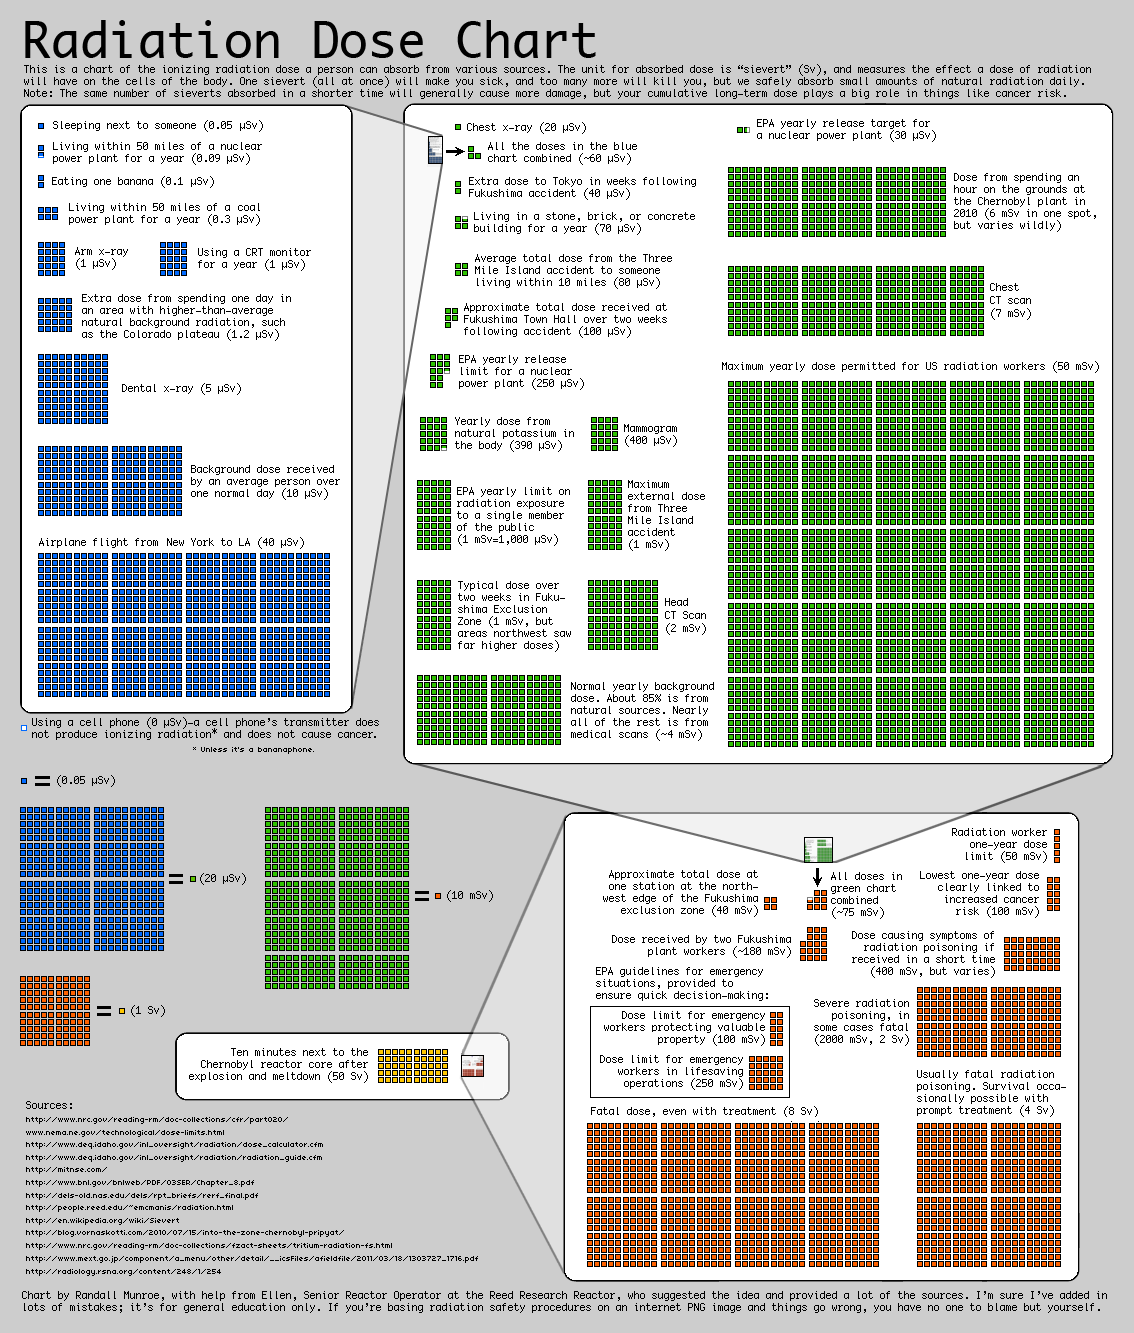
\includegraphics[width=\textwidth]{radioactivity-1/radiation-xkcd}
	\caption{A chart of ionizing radiation dose from various sources. Source: \url{https://xkcd.com/radiation/}}\label{rad1:doses}
\end{figure}

\textbf{Rubrics to focus on during this experiment:} C1, C4, C7, C8, F1, F2, G2. See Appendix~\ref{cha:rubrics} for details.

\subsection{Theory of counting statistics}

If you've ever worked in a not-too-busy retail environment, you’ve probably had the
experience of realizing (perhaps) that random and uniform are two quite different things.
You no doubt have sat waiting for customers, with nobody around for long stretches of
time, and then, as though they'd coordinated in advance, a half dozen people all show up
within a few minutes of each other. Each customer is indeed independent (no, they didn't
have a Twitter call to organize a flashmob!\footnote{Yes, popular interest in flash mobs peaked in 2011. Bear with us here.}) yet their arrival times clearly appear clustered. They are, in fact. But randomly. Uniform – one customer each minute – is quite dramatically different than a random procedure that yields one customer per minute on average. Retail customers (to a great extent), and elementary particles, act randomly, not uniformly.

Each atom in a radioactive sample has, per unit time, some probability of undergoing
radioactive decay. That probability is independent of all the other atoms in the sample.
Each atom decays, or not, based on its own probability and no other. The ensemble of
particle decay counts that one would measure in the sample (using a Geiger counter as we will
do, for example) is described by the something called the Poisson distribution, which
gives, in this instance, the probability of a integer number of events occurring in a fixed
interval of time, given an average rate. For large count rates, like we have here, the
Poisson distribution is indistinguishable from the normal distribution (that is, a simple
Gaussian function).

Specifically, for a process that produces an average $\bar{N}$ counts in a certain time duration (in the case of large $N$), the expected measurement of that count for that time duration is a
random draw from a normal distribution with mean $\bar{N}$ and a standard deviation of
$\sqrt{N}$.

\subsection{Doing the experiment}

\begin{enumerate}
	\item To find the steps of a testing experiment, review Rubric C, found in Table~\ref{rubric:c}.
	
	\item\label{rad1:step:predict-random} A prediction is what the hypothesis says will happen in the event of a particular experimental procedure. Given the hypothesis stated in the goal, and the theory described above, if you collect a series of counts of radioactive decay, what does the hypothesis predict the standard deviation of those counts should be equal to? Record this prediction in your lab notebook.
	
	\item \textbf{Collecting data.} In order to find the standard deviation of a number of measurements, you will need to take those measurements. In the following steps, you will do 10 trials of measuring the count rate (counts per unit time) during periods of about 30 seconds, then take the standard deviation of those 10 trials. Since you will not be able to stop the counter after exactly 30 seconds, you will divide the displayed count by the displayed time to get a count rate (in units of ``counts per second'').
	
	\begin{framed}
		\textbf{The Apparatus.}
		
		For this lab and the following one, you will be provided with a number of different radioactive materials packaged in small plastic disks. Note that each disk has the name of
		the isotope (e.g.\ $^{60}$Co), the type of radiation, and the half-life printed on one side of the
		sample. Half lives can range from fractions of a second to billions of years, depending on
		the isotope.
		
		The energetic particles produced in radioactive decay reactions can be detected by a
		device called a Geiger counter. This consists of a tube filled with inert gas with a wire
		running through it. A high voltage is applied between the wire and the tube. When a high-
		energy particle enters the tube, it can ionize the gas. The freed electrons produce a brief
		pulse of current at the output of the device. The pulses can then be counted.
		
		The counter itself is controlled using buttons on the front panel. \texttt{COUNT} begins the count
		and starts the timer, \texttt{STOP} pauses the count and timer, and \texttt{RESET} sets the count and
		timer to zero. Use the dial on the counter to change the display between the count and the
		elapsed time. When you first turn on the Geiger counter you need to set the voltage to
		$1000\:$V --- the TA will demonstrate how. \textbf{Caution:} Do not turn off the voltage during the
		experiment; use the \texttt{STOP} button to stop the count. \textbf{Do not touch the window on the
		bottom of the tube, as it breaks extremely easily.}
	\end{framed}
	\begin{enumerate}
		\item Take one of the $^{137}$Cs disks and place it printed side down in the plastic shelf shaped to hold it, and place that shelf in the slot second from the top in the stand under the Geiger counter. Note that if you have the Geiger counter on, that it is measuring a large count rate.
		
		\item Use the controls \texttt{COUNT}, \texttt{STOP}, and \texttt{RESET} to measure the number of counts in 10 approximately 30-second intervals. Use the dial on the display to access both the counts and the elapsed time. The provided stopwatch may also help you organize your effort --- \textit{but use the time from the Geiger counter apparatus directly} for your calculations.
		
		\item Record the counts and elapsed time in each interval in a spreadsheet and calculate the count rate in counts per minute (``cpm'' for short).
	\end{enumerate}

	\item \textbf{Analysis.} Note that the count rate is not identical in each trial, even though you accounted for the different measurement durations. Let's see how far away the standard deviation here is from the prediction in Step\ref{rad1:step:predict-random}. Calculate the standard deviation of these measurements. How close is it?
	
	\item Qualitatively, it might appear close or far away, but to test the hypothesis, you should take into account the uncertainty of the standard deviation. This is, effectively, the \textit{standard deviation of the standard deviation}. You would need to take, for example, 10 trials of these 10 trials and compute the standard deviation of that. Fortunately, you have other lab groups who are doing the same experiment. Share the standard deviation you found with the other lab groups, calculate the average and standard deviation of those standard deviations, and use Appendix~\ref{unc:sec:comparing} to compare your average standard deviation to the prediction that your hypothesis made.
	
	\item Use this quantitative comparison to determine if the prediction and the outcome agree or not.
	
	\item Based on that agreement, and taking into account the experimental conditions, make a judgment about the hypothesis.
\end{enumerate}
%\chapter{Radioactive Half-Life}

%TODO add instructor note: to close door to KPTC 003, need to toggle switch that keeps it open, which is above the door.

%TODO add notes about neutron howitzer from https://wiki.uchicago.edu/display/phylabs/Mass+of+the+Neutron and from this email from David McCowan:
%The source is a mixture of plutonium and beryllium. The plutonium decays via alpha emission and the beryllium absorbs the alpha to become carbon + a free neutron. The neutron has an energy given by a very complicated distribution, but the energy distribution goes up to ~11 MeV. The paraffin shielding (and the lucite in the plug) slows down neutrons, so that anything which escapes is thermalized such that E ~ kT ~ 1/40 eV. At the point where the foils are placed, the neutrons have been slowed some, but not completely... if they are a full 11 MeV still, they are too energetic to bind with the silver, so the foils are absorbing from the lower end of the spectrum or from neutrons that have scattered enough material to have less energy than they started with.
%
%The activity of the Pu-Be core is an astounding 5 Ci (!!), but that's the alpha flux which doesn't penetrate out of the core. The neutron flux is considerably less. Looking back at the original purchase order, it looks like we have 80 g of plutoinium mixed with 41 g of beryllium and a listed (I think unshielded?) emission rate of 9 x 10^6 N/sec.

%TODO include suggestion to video the counter and a stopwatch to get more accurate 30-sec readings.

Building on our work from last week, we will continue to study the radioactive decay.
The physical laws of radioactivity predict that the rate of decay (number of atoms
decayed / time interval) is proportional to the number of radioactive nuclei present. This
is due, as we saw in counting statistics previously, to the independence of the decay of
each atom in the sample. The proportionality constant that describes the decay rate
depends on the specific radioactive nucleus. A concise and suggestive way to
characterize the nucleus is by its half-life, the time it takes for the number of radioactive
nuclei to decrease to half of the initial value. You will obtain data to check the form of
the law and to determine the half-life of one or more isotopes of silver.

We will use a device known as a neutron ``Howitzer''. It consists of a source of alpha
particles and a material that absorbs alpha particles and immediately decays by emitting
neutrons. (The neutrons shoot out from the barrel of the shielded volume, vaguely like
shells from WWI artillery, hence the name.)

\section{Background}

We will let the neutrons bombard a small sample of the stable isotope of silver, $^{107}$Ag, to
produce $^{108}$Ag, via the reaction
\begin{equation}
 ^{107}\textrm{Ag} + \mathrm{n} \rightarrow\, ^{108}\textrm{Ag} + \gamma \,,
\end{equation}
where $\mathrm{n}$ represents a neutron and $\gamma$ a gamma particle --- that is, a high energy photon.

The radioactive isotope of silver, $^{108}$Ag, spontaneously decays to an isotope of cadmium
with the same mass number, $^{108}$Cd, by the reaction
\begin{equation}
 ^{108}\textrm{Ag} \rightarrow\, ^{108}\textrm{Cd} + \mathrm{e}^- + \gamma \,,
\end{equation}
where $\mathrm{e}^-$ is an electron (that is, a $\beta$ particle, as we saw and measured last week).

Your TA will bombard silver foils with neutrons using the neutron howitzer. Some of the
nuclei in the foil will have captured a neutron and transformed into a different isotope
which is unstable and can be detected via their decay products. Each group will be given
one of these silver foils.

\section{Procedure}

\textbf{Rubric rows to be assessed:} D1, D4, F1, F2, G2, G3 (ignore actually doing it), G4

Your task is to measure the half-life of $^{108}$Ag. We will use the Geiger tube to count
decays. That is, we will count the $\beta$ particles --- the gamma rays make only a small
contribution to the counts in this instance. You should attempt to carry out the counting
fairly quickly after the silver foil is removed from the howitzer as the decay time is quite
short.

Before the neutron irradiation begins you will want to record the background rate. Press
\texttt{STOP} and \texttt{RESET} on the counter to set the display to zero. Next, press \texttt{COUNT} with no
sample below the Geiger tube and collect the total number of background counts, $N_\textrm{bkg}$ ,
that accumulate in approximately 5 minutes. Once 5 minutes has elapsed press \texttt{STOP} to
end the count. Turn the dial to \texttt{TIME} and record a precise measurement of the elapsed
time, $t$, in seconds. The background rate $R_\textrm{bkg}$ is found with
\begin{equation}
R_\textrm{bkg} = N_\textrm{bkg} /t
\end{equation}
with an uncertainty given by Poisson statistics. Report both the background rate and uncertainty in your lab report.

While the samples are being irradiated, set up your measurement apparatus. Once the samples are ready, quickly place a silver foil sample in the tray below the Geiger tube. Using a stopwatch and the
counter, record the number of counts and the time at 30 second intervals for
about 10 minutes, continuously. Unlike last week's lab with the same apparatus, you will
be recording data continuously, and so will need to use the watch to record times rather
than timer built into the Geiger counter. Record your data.

\section{Calculations}

The experimental data will be used to determine a half-life (or half-lives). We know that
the decay rate ($R=\Delta N / \Delta t$) of a radioactive nuclide is proportional to the number of nuclei present. The proportionality constant is called the decay constant $\lambda$, and the equation that describes what was just discussed is
\begin{equation}
 R = \lambda N \,,
\end{equation}
where $N$ is the background-subtracted counts. Using integral calculus and the above equation, we find
\begin{equation}
 N = N_0 e^{-\lambda t} \,,
\end{equation}
where $N_0$ is the number of nuclei at the initial time $t=0$. The half life $T_{1/2}$ is defined by
the time it takes for $N = N_0 /2$ and is related to the decay constant by $T_{1/2} = \ln(2)/ \lambda$, where
$\ln()$ is the natural logarithm function, and so $\ln(2) \approx 0.693$.

We can now write the radioactive decay equation as
\begin{equation}
 R = \lambda N_0 e^{-t \ln(2) / T_{1/2}} \,.
\end{equation}
Taking the logarithm of both sides and substituting for $N$ gives
\begin{equation}
 \ln(R) = - \left(\frac{\ln(2)}{T_{1/2}} \right) t + \mathrm{const} \,.
\end{equation}
Your TA will help you to understand the details of this derivation.

Make a plot showing $\ln(R)$ on the vertical axis and elapsed time, $t$, along the horizontal
axis. Don’t forget to subtract the background where appropriate. Calculate the slope
and use this value to solve for the half life using the above equations. Report this value
along with a table of your decay rate data and the plot described above.

\section{Questions (these should be included in your lab report)}

\begin{enumerate}
	\item Look up the half-lives of the various nuclides of silver. What is the published
	half-life of the nuclide you’re observing? How does this compare with your
	calculated result? Calculate the percent difference in your result.
	
	\item For the silver foil, how long would it take before you would expect to detect only
	one count per second, background corrected?
	
	\item The detector only measures particles that travel up into the detector. The majority
	of particles traveling in the other directions escape detection. Will this short-
	coming affect the measured half-life? If so, how? If not, why not?
	
	\item Describe one thing you could change in this experiment that could lead to a more
	accurate measurement of the half-life of the silver isotope.
	
	\item The particular irradiated silver sample you used contained some unknown
	percentage of the unstable silver isotope, and was irradiated at some unmeasured
	time before you began your experiment. Does this matter to your results? Explain.
	
\end{enumerate}
%\chapter{Local Gravitational Field}

One of Newton's revelations was that physical laws that governed the movement of objects near Earth also predicted the movements of objects in the sky.
The apocryphal story of an apple falling on Newton's head brings to mind the mechanism of gravity --- the phenomenon of massive objects attracting each other.
In this lab, you will measure the strength that gravity has where we are, near the Earth's surface. This measurement might also enable us to learn more about the mass of the Earth itself in a future lab.

\section{Learning goals}

\begin{itemize}
	\item Understand Newton's law of universal gravitation and its linear approximation
	
	\item Identify sources of statistical and systematic error
	
	\item Demonstrate an ability to make careful measurements
	
	\item Demonstrate proficiency in basic calculations and plotting
	
	\item Explain the importance of repeated measurements and sufficiently large datasets
	
	\item Use experimentally derived quantities to obtain a mass for the Earth.
\end{itemize}

\section{Scientific Background}

\subsection{The gravitational field strength and Newton's second law}

The force of gravity, $F$, between two objects with mass $m_1$ and $m_2$ and whose centers are separated by a distance $R$ is given by Newton's law,
\begin{equation}\label{lg:eq:newtons}
 F_\textrm{gravity} = G \frac{m_1 \: m_2}{r^2} \,,
\end{equation}
where the Newtonian constant of gravitation $G = 6.67408(31) \times 10^{-11} \: \textrm{m}^3 \: \textrm{kg}^{-1} \: \textrm{s}^{-2}$. Astronomers apply Newton's law to infer fundamental information about astrophysical objects, for example the mass of binary stars. Indeed, this is one of the most common methods by which astronomers ``weigh'' astrophysical objects, including the Earth itself. For measuring the force acting on an object of mass $m$ that is affected predominantly by the Earth's gravity, the force acting on it would be
\begin{equation}\label{lg:eq:fearth}
 F_\textrm{Earth} = \frac{G M_\Earth}{(R_\Earth + h)^2} m
\end{equation}
where $M_\Earth$ and $R_\Earth$ are the mass and radius of the Earth, respectively, and $h$ is the height above the Earth.

For objects near the Earth's surface, where $h$ is much less than $R_\Earth$, $h$ can be treated as zero, resulting in a constant gravitational force, with Equation~\ref{lg:eq:fearth} reducing to
\begin{equation}\label{lg:eq:fearthred}
F_\textrm{Earth} = \frac{G M_\Earth}{(R_\Earth)^2} m \,.
\end{equation}
Notice that on the right-hand-side of this equation, the only variable is the mass. The others, together, constitute the \textit{strength of the local gravitational field}, $g$ (sometimes pronounced ``little g''). So our simplified equation is
\begin{equation}\label{lg:eq:fegm}
 F_\textrm{Earth} = g m \,,
\end{equation}
where we have made the substitution
\begin{equation}\label{lg:eq:g}
g = \dfrac{G M_\Earth}{(R_\Earth)^2} \, .
\end{equation}
Notice that we have taken a complicated inverse square equation (Equation~\ref{lg:eq:fearth}) and
converted it to a much simpler one (Equation~\ref{lg:eq:fegm}). This process is called \textit{linearization} and is a
trick astronomers often use to make calculations more manageable. You will encounter
this technique throughout this and other PHSC courses.

We see from Equation~\ref{lg:eq:g} that if we can make accurate measurements of $g$, $G$, and $R_\Earth$, we can calculate the mass of the Earth. We'll look up $R_\Earth$ online, and next week we will measure $G$. To find $g$, we note that Newton's second law of motion states that the acceleration $a$ of an object is directly proportional to the net force $F_\textrm{net}$ acting on it and inversely proportional to its mass, $m$, or, more succinctly and slightly rearranged,
\begin{equation}
 F_\textrm{net} = m a \,.
\end{equation}
If the Earth's gravity is the only force acting on our object, then $F_\textrm{net} = F_\textrm{Earth}$, and substituting Equation~\ref{lg:eq:fegm}, we find that
\begin{equation}
 g m = m a \,,
\end{equation}
and thus, simplifying,
\begin{equation}
 a = g \,.
\end{equation}
So, the acceleration of an object that is subject only to the Earth's gravity is equal to the local gravitational field strength. If we can measure the acceleration, then we can find $g$, and get one step closer to determining the mass of the Earth.

\subsection{Constantly accelerated motion}

If an object is subject to a constant force, then according to Newton's second law, it undergoes constant acceleration. If an object undergoes constant acceleration $a$, and we know the object's initial position $x_0$ and velocity $v_0$, then after a time duration $t$, we can derive using calculus that the object's position $x$ and velocity $v$ are given by
\begin{equation}\label{lg:eq:x-const-a}
 x = x_0 + v_0 t + \frac{1}{2} a t^2
\end{equation}
and
\begin{equation}
 v = v_0 + a t \,.
\end{equation}

\section{Application experiment: determine $\bm{g}$ on the Earth's surface}

\textbf{Goal:} Determine $g$ near the Earth's surface by finding the acceleration of an object undergoing freefall (no substantial forces other than gravity) using two different methods: 

\textbf{Rubrics to be assessed:} D4, D5, F1, F2, G1, G2, G4

\textbf{Available equipment:} stopwatch, dense object to drop, meter stick, camera (including the one on your phone), computer with Tracker\footnote{Open Source Physics Tracker can be downloaded from \url{https://physlets.org/tracker} and is also installed on the lab computers.} installed.

\subsection{Method 1: freefall time}

\begin{enumerate}
	\item Drop the object from a known height and measure the time to fall with a stopwatch. Do this as many times as makes sense to you.
	
	\item List the sources of uncertainty and determine whether each is a random uncertainty or an instrumental uncertainty.
	
	\item Calculate the average fall time.
	
	\item Calculate the standard deviation of the average fall time (using Equation~\ref{unc:eq:stdevmean}), and report the latter as the uncertainty in the average fall time.
	
	\item Use the average fall time and the initial position and velocity of the object to calculate the acceleration.
	
	\item Propagate the uncertainty in the time and position to find the uncertainty of your measured acceleration (see Section~\ref{unc:sec:prop})
	
	\item Report the acceleration found by this method as ``value $\pm$ uncertainty [units]''. For example, $9.73 \pm 0.04\:$m/s$^2$.
\end{enumerate}

\subsection{Method 2: Video tracking}

It is helpful to use two methods to find the same quantity, so that mistakes or incorrect assumptions made in one method do not carry over to the other, and are thus more likely to be detected. In this method, you will record a video of an object falling, make a position vs. time plot, and fit the constant acceleration equation (Equation~\ref{lg:eq:x-const-a}). You will use a computer program to make this analysis easier.

\subsubsection{Record the video}

\begin{enumerate}
	\item Find a good object to drop. It should be dense enough to not be slowed down significantly by air resistance.
	
	\item Using the camera on one of your group member's phones, record a video of the object falling.
	
	Here are some tips to get a quality video:
	\begin{itemize}
		\item Include an object of known length in the shot, at the same distance from the camera as the falling object. This gives a reference length, so that you can find how each camera pixel scales to the physical situation.
		
		\item Avoid parallax error by having the object be at about the same distance from the camera throughout the fall. Having the camera be farther away can help. Also, you can ensure that the top and the bottom of the fall are the same distance from the camera.
		
		\item Hold the camera steady.
	\end{itemize}

	\item Record that video and transfer the video to a computer that has Tracker installed.
\end{enumerate}

\subsubsection{Importing the data into Tracker}

In this part, you'll use Tracker to record the position of the object at each timestep. To do this, you'll need to tell it what direction ``down'' is in, what the scale of the image is, and when time $t=0$ is. Then you'll record the positions, find out what parameters best fit the curve that is produced, and use those to find the acceleration.

\begin{enumerate}
	\item Open Tracker on a computer. You can install it on your own computer by visiting \url{https://physlets.org/tracker}.
	
	\item In Tracker, open your video.
	
	\item \textbf{Find frame when zero time is.} Move the slider below the video to the right to advance the frames until you find the first one in which the object is falling. Record that start frame number, which is found to the left of the slider bar in red.
	
	\item \textbf{Find the last relevant frame.} Keep moving the slider to the right until you find the last frame before the object hits the floor. Record that end frame number.
	
	\item To \textbf{tell Tracker about these frames}, click the 5th icon from the left on the toolbar above the video (``Clip settings'') and enter the start frame and end frame.
	
	\item \textbf{Tell Tracker how long things are.} In astronomy applications, this is known as the ``pixel scale''. Here we can just draw a line on the frame and tell Tracker how long that line is in real life. Click the 6th icon from the left (blue, with a ``10'') and select \texttt{New} $\rightarrow$ \texttt{Calibration Stick}. Shift-click to mark each end of your known length, and type in your known length, with units in the box that appears along the stick. Use ``m'' for meters.
	
	\item \textbf{Align the coordinate system.} In the toolbar, click the 7th icon from the left (magenta crossed lines). Click and drag the coordinate system's origin (the intersection of long lines) to the location of the object in the start frame.
	
	\item \textbf{Check to see if the camera was tilted.} Advance the video to see if the object moves along an axis. If it goes off at an angle, the camera was tilted compared to the direction of motion. In this case, rotate the coordinate system to align with the motion by clicking and dragging the small line that crosses one of the axes.
	
	\item \textbf{Tell Tracker where the object is in every frame.}
	\begin{enumerate}
		\item In the toolbar, click \texttt{Create} $\rightarrow$ \texttt{Point Mass}.
		\item Ensure the slider is at the start frame.
		\item Shift-click on the object. Notice that the frame advances to the next one automatically.
		\item Continue to shift-click to mark the object's position throughout the duration.
	\end{enumerate}
\end{enumerate}

\subsubsection{Analysis}

\begin{enumerate}
	\item \textbf{Ensure the correct axis is selected for analysis.} Look at the plot to the right of the video. If there is not a smooth-ish curved line, click on the axis label ``x (m)'' and choose instead ``y (m)''.
	
	\item In the drop-down menu, select \texttt{View} $\rightarrow$ \texttt{Data Tool (Analyze...)}.
	
	\item In the window that appears, above the plot, click \texttt{Analyze} $\rightarrow$ \texttt{Curve Fits}.
	
	\item Notice that Eq.~\ref{lg:eq:x-const-a}, which describes freefall, is a quadratic equation, which means the shape is a parabola. For ``Fit Name'', choose ``Parabola'' from the drop-down menu.
	
	\item Use the Fit Equation and Parameter Values, comparing with Equation~\ref{lg:eq:x-const-a}, to find the acceleration $a$, and thus the gravitational field strength $g$.
	
	\item To get an uncertainty for this value, use the ``rms dev'' value, which describes the average deviation of the fit equation from the points, divide that by the average (mean) position, and multiply that by your value for the acceleration. You can find the mean position by selecting \texttt{Analyze} $\rightarrow$ \texttt{Statistics} and reading above the data table column.
\end{enumerate}

\subsection{Comparing the methods, final determination of $\bm{g}$}

\begin{enumerate}
	\item Compare the values of $g$ from the two methods using the $t'$ statistic as described in Appendix~\ref{unc:sec:comparing}.
	
	\item Use that comparison and your assessment of which method had fewer questionable assumptions to decide on your final answer for $g$ (including an uncertainty). How close is it to the average $g$ described, for example, on Wikipedia?
\end{enumerate}
%\chapter{Measuring the Gravitational Constant}

Gravity is the least understood of the fundamental forces, and it is the one that is most easily noticed by humans. Part of the reason for this second part is that gravity is weak enough that we can easily push and move against it (for example, walking or launching a rocket). Compared with the electromagnetic bonds that are holding molecules together or the nuclear forces that hold atomic nuclei, gravity is extremely weak.

If it is universal, though, we should be able to measure the gravitational attraction between any two massive objects, if we are very careful and have sensitive equipment. In this lab, we will measure the gravitational force between lead spheres and use that to find the Newtonian constant of gravitation, $G$, which is a measure of how strong, in general, the force of gravity is.

\section{Learning goals}

\begin{itemize}
	\item Follow the procedure of an important physical measurement.
	
	\item Identify sources of statistical and systematic error.
	
	\item Demonstrate an ability to make careful measurements.
\end{itemize}

\textbf{Rubrics rows to be assessed:} D4, D8, F1, F2, G1, G2, G4.

\section{Scientific Background}

In 1798, Henry Cavendish completed his measurements of ``the density of Earth'' using a
simple yet extremely sensitive apparatus: a torsion balance. He placed a small lead sphere
of mass $m = 0.73\:$kg at each end of a wooden rod, which was suspended horizontally.
Two large lead spheres, each of mass $M = 159\:$kg, were fixed in place, at a distance $R =
23\:$cm from each of the smaller spheres. When the torsion balance was released and
allowed to move freely, the lead spheres would be attracted by the gravitational force according to Newton's law of universal gravitation,
\begin{equation}\label{cav:eq:newtons-grav}
 F = G \frac{M m}{R^2} \,.
\end{equation}
To protect the balance from air currents and temperature changes, Cavendish placed it in
a closed room (Fig.~\ref{cav:fig:original-setup}), appropriately equipped for remote operation and reading of the
torsion angle.

\begin{figure}
	\centering
	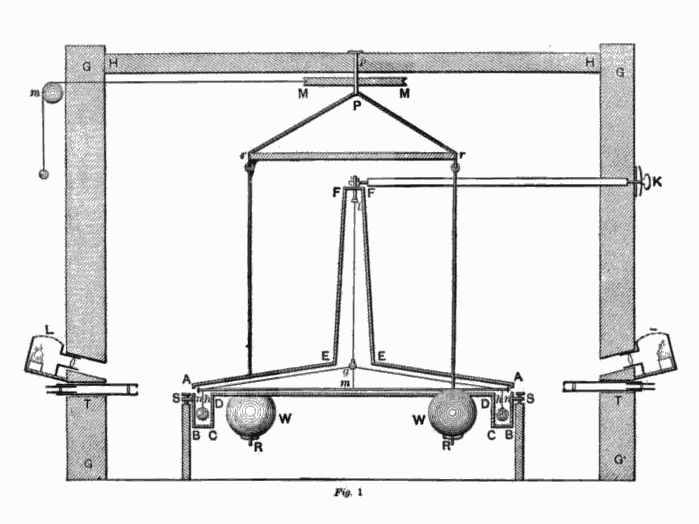
\includegraphics[width=\textwidth]{cavendish/Cavendish_Experiment}
	\caption{Henry Cavendish's sketch of his experimental setup.}\label{cav:fig:original-setup}
\end{figure}

While Cavendish's main objective was the measurement of the density of Earth, in fact
he had performed a measurement of the Gravitational constant $G$ to a remarkable
accuracy ($\approx 1\%$).

High precision torsion balances are still used nowadays to test fundamental principles of
general relativity (the equivalence of the inertial and gravitational mass) and possible
deviations of the Newton’s law of gravitation. In this lab, you will measure the
Gravitational constant with a modern version of the Cavendish torsion balance.

\section{Apparatus and Theory}\label{cav:sec:apparatus}

The setup and measurement of the Gravitational constant is conceptually straightforward (Fig.~\ref{cav:fig:setup-booms}). A boom
with two small, identical lead spheres (labeled `A' in the figure) of mass $m$ is suspended by a thin tungsten
wire. Since the masses are identical, the system is in equilibrium under the Earth
gravitational field. At a certain moment, two large lead spheres (B) of mass $M$ are placed
close to the A spheres.

\begin{figure}
	\centering
	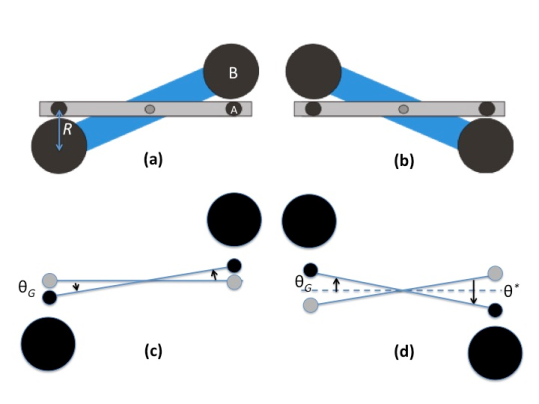
\includegraphics[width=0.7\textwidth]{cavendish/tel-rp2111-booms}
	\caption{A torsion balance. In (a) and (b), top view of the Cavendish balance with two
		symmetric configurations of the lead spheres. In (c) and (d), the corresponding
		equilibrium positions and rotation angles.}\label{cav:fig:setup-booms}
\end{figure}

The gravitational force between spheres A and B is given by Eq.~\ref{cav:eq:newtons-grav}. This force induces a torque $\tau_G$ on the boom which starts to rotate. From the laws of
physics, the torque is given by
\begin{equation}
 \tau_G = 2 F_G d \,
\end{equation}
where $d$ is the distance to the center of A from the center of the boom (the factor 2 comes
from the fact that there are two B spheres each exerting a force $F_G$). The suspending
wire, which is fixed at its top end, is twisted by the rotation of the boom (Fig.~\ref{cav:fig:torsion}), and
``tries'' to recover its initial position by a counter-torque $\tau_w$. For a small rotation angle $\theta$,
$\tau_w$ is proportional to $\theta$,
\begin{equation}
 \tau_w = k \theta\,,
\end{equation}
where the torsion constant $k$ depends on the wire's material and dimensions.

\begin{figure}
	\centering
	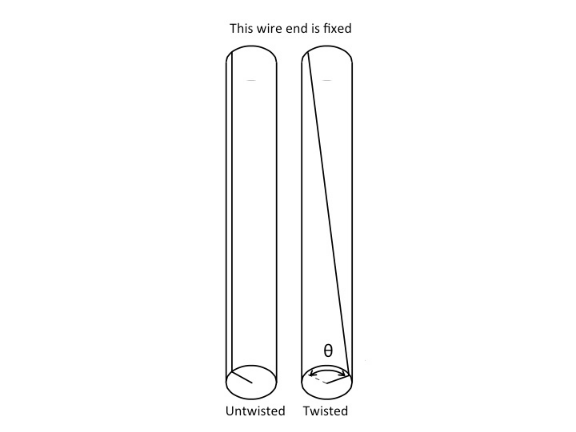
\includegraphics[width=0.8\textwidth]{cavendish/torsion-balance}
	\caption{Twisted wire of a torsion balance.}\label{cav:fig:torsion}
\end{figure}

A new equilibrium position is achieved when the boom has rotated by an angle $\theta_G$ (Fig.~\ref{cav:fig:setup-booms}(c)) such that the two torques equilibrate themselves, so
\begin{equation}\label{cav:eq:equal-taus}
\tau_G = \tau_w \,.
\end{equation}
From Eqs.~(\ref{cav:eq:newtons-grav}--\ref{cav:eq:equal-taus}), the gravitational constant is obtained:
\begin{equation}\label{cav:eq:final-g}
G = \frac{k \theta_G R^2}{2 M m d}\,.
\end{equation}

The symmetry of the torsion balance can be exploited to perform a more precise
measurement of rotation angle $\theta_G$ (which is very small). After the boom has reached the
equilibrium in the Fig.~\ref{cav:fig:setup-booms}(c) configuration, the B spheres are placed in the symmetric position of Fig.~\ref{cav:fig:setup-booms}(b), which results in a new equilibrium position as in Fig.~\ref{cav:fig:setup-booms}(d).
Thanks to the symmetry of the apparatus, the rotation angle $\theta_\textrm{rotation}$ between the two
configurations is simply twice the angle $\theta_G$. With the Cavendish balance described in
Section~\ref{cav:sec:measurement}, you will measure $\theta_\textrm{rotation}$ and then use the following equation to find $\theta_G$:
\begin{equation}\label{cav:eq:theta-g}
 \theta_G = \theta_\textrm{rotation} / 2 \,.
\end{equation}

When performing the experiment, you will notice that the torsion balance undergoes
harmonic oscillations around its equilibrium position. The dampening of the oscillations
(that is, the decrease of their amplitude with time) is due primarily to air dragging against
the boom. The period $T$ of the oscillations depends on the torsion constant $k$ according to
\begin{equation}\label{cav:eq:k}
 k = 2 m d^2 \left( \frac{2 \pi}{T} \right)^2 \,.
\end{equation}
Note that the quantity $2 m d^2$ is the \textit{moment of inertia} of the A spheres.

\section{Procedure: Measurement of $\bm{G}$ with the Cavendish Balance}\label{cav:sec:measurement}

You will perform a measurement of the Gravitational constant using data taken with a
computerized Cavendish balance (Fig.~\ref{cav:fig:comp-setup}). The apparatus is placed on a wooden box filled
with sand which helps in dampening vibrations (of the building, when you walk close to
the apparatus, etc.). The rotation angle is measured by a ``differential capacitive sensor''
which provides a more stable and convenient way of recording when compared to other
methods (e.g. using a laser). The apparatus is extremely sensitive and requires several
hours of preparation. For this reason, it is not possible to set it up and take good data
during a standard two-hour lab session. Thus, you will find the apparatus ready for the
measurements, which will be performed by the TA by moving the B spheres in the two
configurations of Fig.~\ref{cav:fig:setup-booms}. You will notice that after the TA has moved the spheres, the
boom will start to oscillate and it will take about one hour for the oscillations to dampen
around a new equilibrium position. The TA will then provide you with the data after the
session. Sometimes the data collected during your session will not be of good enough
quality for the measurement (this is indeed a very difficult experiment and we are trying
to do it while you walk around the room causing vibrations), and in such case you will
be provided a set of data from another session. An example of data is given in Fig.~\ref{cav:fig:data}
(your data will be significantly noisier).

\begin{figure}
	\centering
	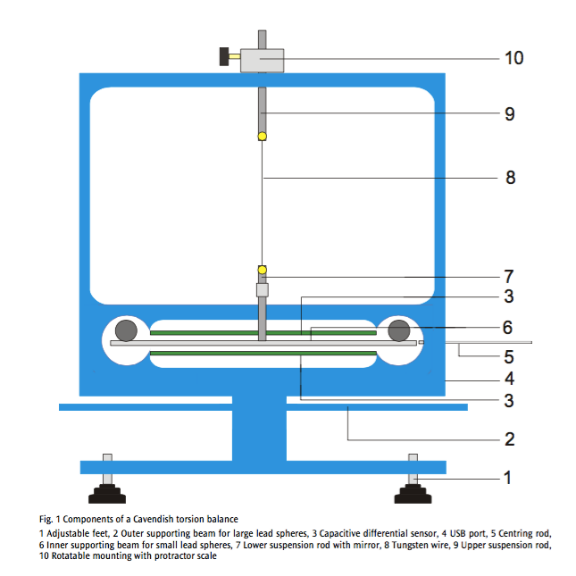
\includegraphics[width=\textwidth]{cavendish/tel-rp2111-setup}
	\caption{The computerized Cavendish balance.}\label{cav:fig:comp-setup}
\end{figure}

\begin{figure}
	\centering
	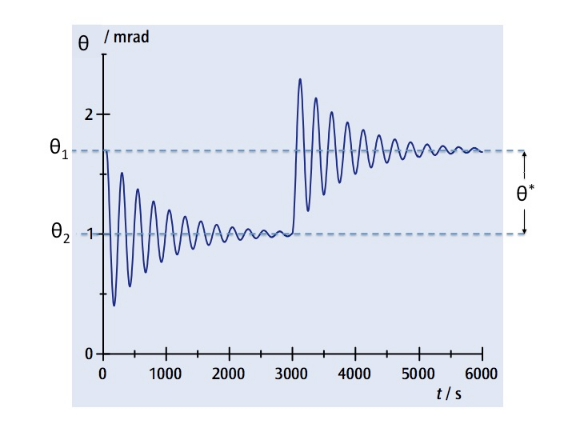
\includegraphics[width=0.8\textwidth]{cavendish/tel-rp2111-example-data}
	\caption{Example of data from the Cavendish balance.}\label{cav:fig:data}
\end{figure}

By analyzing the data, you can determine the Gravitational constant with the following
procedure:
\begin{enumerate}
	\item Measure the period $T$ of oscillation (e.g. by measuring the time between two
	consecutive maxima of the damping oscillations), and determine $k$ using Eq.~(\ref{cav:eq:k}). For a more
	accurate measurement of $T$, measure the time corresponding to several
	oscillations and divide it by the number of oscillations. Use Fig.~\ref{cav:fig:geo} for the values
	of the masses and the geometrical parameters.
	
	\item Measure the rotation angles $\theta_1$ and $\theta_2$ corresponding to the equilibrium positions
	of the first and second oscillation, respectively (see Fig.~\ref{cav:fig:data}). Try various ways to measure the rotation angles (e.g. fitting by eye an horizontal line; sum the
	maxima and minima of consecutive oscillations). You can then calculate
	\begin{equation}
	\theta_\textrm{rotation} = \abs{\theta_1 - \theta_2}
	\end{equation}
	and use Eq.~(\ref{cav:eq:theta-g}) to derive $\theta_G$.
	
	\item Determine the gravitational constant G using Eq.~(\ref{cav:eq:final-g}) and compare your result with its nominal value.
	
	\item Note that the mathematical procedure given here makes some assumptions about what is important to include. Discuss with your group to identify those assumptions and report these in your report.
\end{enumerate}

\begin{figure}
	\centering
	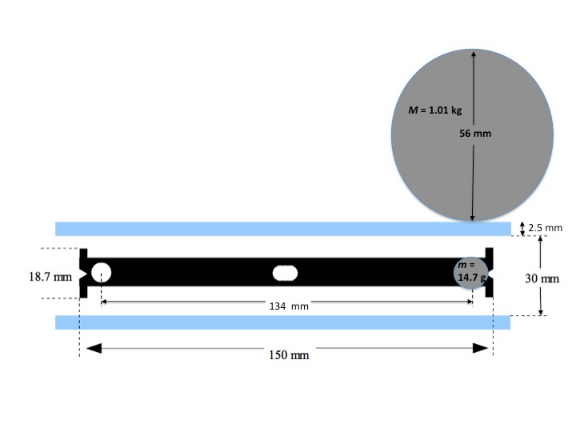
\includegraphics[width=\textwidth]{cavendish/tel-rp2111-geometry}
	\caption{Geometry of the Cavendish balance and lead spheres masses.}\label{cav:fig:geo}
\end{figure}

\section{Procedure: Build the Cavendish Balance}

While the computerized Cavendish balance is acquiring data, you will build and calibrate
a similar apparatus. This part of the lab will give you a deeper understanding of the
Cavendish balance, and a hands-on experience on the extreme sensitivity of the
apparatus. A description of the PASCO balance and instructions are given in the manual in Appendix~\ref{cha:pasco-cavendish}.
Read pages 1--3 of the manual and familiarize yourself with the different components of
the balance.

\begin{enumerate}
	\item First, mount the thin tungsten wire which will be used to suspend the
	pendulum bob. The mounting mechanism is shown in Figs.~\ref{cav:fig:pasco-block}--\ref{cav:fig:pasco-assembly}. A good eye,
	cooperation within you group, and patience is required for this step; be careful in
	handling the wire since it can break (and probably will until you get enough
	practice).
	
	\item To install the wire, screw the small aluminum block onto the tab as in Fig.~\ref{cav:fig:pasco-block} (you
	need to assemble two of these pieces).
	
	\item Mount one of them on the brass rod (torsion wire head) as in Fig.~\ref{cav:fig:pasco-assembly}.
	
	\item Cut $\approx 50\:$cm of wire from the spool; be careful in keeping the wire straight
	avoiding kinks.
	
	\item Take one end of the wire, slide it between the aluminum block and the plate
	(slightly loosen the screw to let the wire in) and make a loop around the screw;
	tighten the screw while keeping the wire (and the aluminum block) straight.
	
	\item Take the other end of the wire and do the same with the other mounting piece; the
	length of the wire between the two mounting screws must be $37.5\:$cm (Fig.~\ref{cav:fig:pasco-assembly}).
	
	\item Thread the wire through the shaft of the Cavendish apparatus (you may need the
	help of a thin screwdriver to slide the mounting piece in).
	
	\item Using the zero adjust knob (see PASCO manual), align the bottom tab with the
	face of the pendulum bob.
	
	\item Tighten the screw on the top of the balance to secure the torsion wire head.
	
	\item Attach the bottom tab to the pendulum bob using the Philips screw.

\end{enumerate}

\begin{figure}
	\centering
	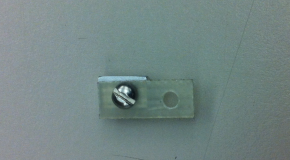
\includegraphics[width=0.5\textwidth]{cavendish/pasco-block}%
	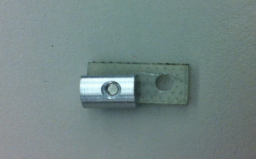
\includegraphics[width=0.45\textwidth]{cavendish/pasco-tab}
	\caption{Wire mounting pieces, aluminum block and tab.}\label{cav:fig:pasco-block}
\end{figure}

\begin{figure}
	\centering
	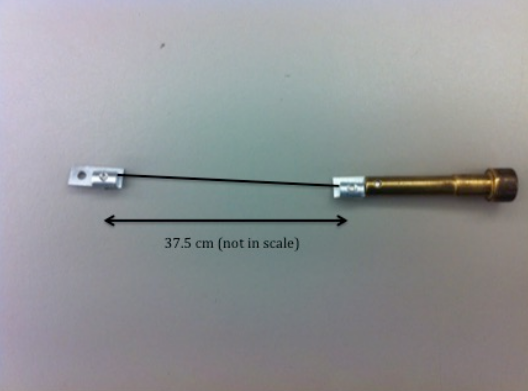
\includegraphics[width=0.7\textwidth]{cavendish/pasco-assembly}
	\caption{Assembly of torsion wire.}\label{cav:fig:pasco-assembly}
\end{figure}

Also, check the Section ``Maintenance'' of the PASCO manual which provides a
description of a similar procedure using a torsion ribbon.

Once you have successfully completed this step, you can proceed to leveling the
Gravitational torsion balance, to perform the vertical adjustment of the pendulum and the
rotational alignment of the pendulum bob arms. Follow the instructions on pages 3--6 of
the PASCO manual. Ask the TA for advice and help if necessary. At the end of the
session, show to the TA which steps you have been able to complete.

\section{Procedure: Measure $\bm{G}$ with the PASCO Cavendish balance}

Once you have your own Cavendish balance built and leveled (see the previous section), you are ready to take your own data.

Since the expected deflection angle $\theta_G$ is on the order of milliradians, measuring it with a protractor directly is not a practical solution (the instrumental uncertainty of a typical protractor is 0.5\textdegree$\approx 9\:$milliradians). Instead, you will direct a laser beam toward a mirror mounted on the pendulum bob and measure the linear displacement of reflected ray on a screen on the other side of the room (the larger the distance to the screen, $L$, the larger the linear displacement $d$ for the same bob deflection angle $\theta_d$, which leads to a smaller uncertainty). Then, you will use that displacement length to calculate that angle, according to
\begin{equation}\label{cav:eq:displacement}
 \theta_d = \frac{d}{2 L} \,.
\end{equation}

Here is a suggested step-by-step procedure:
\begin{enumerate}
	
	\item Ensure that the laser, pendulum, and screen are arranged such that the laser can strike the pendulum mirror and reflect onto the screen, which is set up across the room (the larger the distance, the less uncertainty in the angle determination).
	
	\item Measure and record the distance $L$ from the pendulum to the screen.
	
	\item Rotate the large-mass support arm so that it makes an approximately 90\textdegree angle with the pendulum arm.
		
	\item Setup and level the balance according to pages 3--6 of the equipment manual in Appendix~\ref{cha:pasco-cavendish}, sections Initial Setup, Leveling the Gravitational Torsion Balance, Vertical Adjustment of the Pendulum, and Rotational Alignment of the Pendulum Bob Arms. In this last section, you do not need to be extremely precise about alignment --- aim for ``roughly aligned''. We will correct for any misalignment by using differences in angles, rather than the angles themselves.

	\item Decide how to collect the data. Your aim is to measure the linear displacement of the beam from an arbitrarily marked zero point on the screen, as a function of time. The result should be a table of (time,displacement) values.
	\begin{itemize}
		\item To take data manually, use a stopwatch, meter stick, and teamwork to take data at regular time intervals that are close enough together to capture the periodic motion.
	
		\item To take data with video tracking, record the movement of the laser beam on the screen with a camera whose line of sight is at roughly a right angle to the surface of the screen. Load the video in Open Source Physics Tracker and record the position of the laser similar to the local gravitational field (``little gee'') lab.
	\end{itemize}
	
	\item Quiet the pendulum by following Steps 5a and 5b from page 5 of the equipment manual.
	
	\item Slowly and gently rotate the large-mass support arms counter-clockwise until one of the large spheres is touching the case plate.
	
	\item Collect the data according to your chosen method. Ensure that you record several complete cycles of oscillation.
	
	\item Rotate the large-mass support arms clockwise until a sphere is touching a case plate.
	
	\item Continue collecting data, ensuring that you record several complete cycles of oscillation.
	
	\item Using Tracker or the manual method, create a spreadsheet with columns Time (s) and Displacement (m).
	
	\item Create another column ``Deflection Angle (rad)'' and calculate this angle for each row using Eq.~\ref{cav:eq:displacement}.
	
	\item Follow the numbered steps in Section~\ref{cav:sec:measurement} to calculate $G$ and its uncertainty.
\end{enumerate}

\section{Calculations \& Analysis}

The data acquired by the computerized Cavendish balance are provided as an Excel file,
which also includes a plot of this data. The plot shows rotation angle (in milliradians, where 1 milliradian =
0.001 radians, on the vertical axis) as a function of time (in seconds, on the horizontal axis). Follow
Section~\ref{cav:sec:apparatus} to do the necessary data analysis and measure the gravitational constant $G$. You
will need to measure (1) the period of oscillations $T$ and (2) the rotation angles
corresponding to the two equilibrium positions. You are interested in the difference
between the angles.


\appendix

\chapter{Analysis of Uncertainty}

A physical quantity consists of a value, unit, and uncertainty.
For example, ``$5 \pm 1\,$m'' means that the writer believes the true value of the quantity to most likely lie within 4 and 6 meters\footnote{The phrase ``most likely'' can mean different things depending on who is writing.
	If a physicist gives the value and does not given a further explanation, we can assume that they mean that the measurements are randomly distributed according to a normal distribution around the value given, with a standard deviation of the uncertainty given.
	So if one were to make the same measurement again, the author believes it has a 68\% chance of falling within the range given.
	Disciplines other than physics may intend the uncertainty to be 2 standard deviations.}.
Without knowing the uncertainty of a value, the quantity is next to useless.
For example, in our daily lives, we use an implied uncertainty.
If I say that we should meet at around 5:00 pm, and I arrive at 5:05 pm, you will probably consider that within the range that you would expect.
Perhaps your implied uncertainty is plus or minus 15 minutes.
On the other hand, if I said that we would meet at 5:07 pm, then if I arrive at 5:10 pm, you might be confused, since the implied uncertainty of that time value is more like 1 minute.

Scientists use the mathematics of probability and statistics, along with some intuition, to be precise and clear when talking about uncertainty, and it is vital to understand and report the uncertainty of quantitative results that we present.

\section{Types of measurement uncertainty}

For simplicity, we limit ourselves to the consideration of two types of uncertainty in this lab course, instrumental and random uncertainty.

\subsection{Instrumental uncertainties}

Every measuring instrument has an inherent uncertainty that is determined by the precision	
  of the instrument.
Usually this value is taken as a half of the smallest increment of the instrument's scale. For example, $0.5\:$mm is the precision of a standard metric ruler; $0.5\:$s is the precision of a watch, etc. For electronic digital displays, the equipment's manual often gives the instrument's resolution, which may be larger than that given by the rule above.

Instrumental uncertainties are the easiest ones to estimate, but they are not the only source of the uncertainty in your measured value.
You must be a skillful experimentalist to get rid of all other sources of uncertainty so that all that is left is instrumental uncertainty.

\subsection{Random uncertainties}

Very often when you measure the same physical quantity multiple times, you can get different results each time you measure it.
That happens because different uncontrollable factors affect your results randomly.
This type of uncertainty, random uncertainty, can be estimated only by repeating the same measurement several times.
For example if you measure the distance from a cannon to the place where the fired cannonball hits the ground, you could get different distances every time you repeat the same experiment.	
  
For example, say you took three measurements and obtained 55.7, 49.0, 52.5, 42.4, and 60.2 meters. We can quantify the variation in these measurements by finding their standard deviation using a calculator, spreadsheet, or the formula (assuming the data distributed according to a normal distribution)
\begin{equation}
 \sigma = \sqrt{\sum_{i=1}^{N} \frac{(x_i-\bar{x})^2}{N-1}} \, ,
\end{equation}
where $\{x_1, x_2, \dots, x_N\}$ are the measured values, $\bar{x}$ is the mean of those values, and $N$ is the number of measurements.
For our example, the resulting standard deviation is 6.8 meters. Generally we are interested not in the variation of the measurements themselves, but how uncertain we are of the average of the measurements. The uncertainty of this mean value is given, for a normal distribution, by the so-called ``standard deviation of the mean'', which can be found by dividing the standard deviation by the square root of the number of measurements,
\begin{equation}
\sigma_\textrm{mean} = \frac{\sigma}{\sqrt{N}} \, .
\end{equation}
So, in this example, the uncertainty of the mean is 3.0 meters. We can thus report the length as $52 \pm 3\:$m.

Note that if we take more measurements, the standard deviation of those measurements will not generally change, since the variability of our measurements shouldn't change over time. However, the standard deviation of the mean, and thus the uncertainty, will decrease.

\section{Propagation of uncertainty}

When we use an uncertain quantity in a calculation, the result is also uncertain. To determine by how much, we give some simple rules for basic calculations, and then a more general rule for use with any calculation which requires knowledge of calculus. Note that these rules are strictly valid only for values that are normally distributed, though for the purpose of this course, we will use these formulas regardless of the underlying distributions, unless otherwise stated, for simplicity.

If the measurements are completely independent of each other, then for quantities $a \pm \delta a$ and $b \pm \delta b$, we can use the following formulas:
\begin{equation}\label{unc:add}
\textrm{For } c = a + b \textrm{ (or for subtraction), } \delta c = \sqrt{(\delta a)^2 + (\delta b)^2}
\end{equation}

\begin{equation}\label{unc:mult}
\textrm{For } c = ab \textrm{ (or for division), } \frac{\delta c}{c} = \sqrt{\left(\frac{\delta a}{a}\right)^2 + \left(\frac{\delta b}{b}\right)^2}
\end{equation}

\begin{equation}\label{unc:exp}
\textrm{For } c = a^n,\, \frac{\delta c}{c} = n \frac{\delta a}{a}
\end{equation}

If you are familiar with calculus, you may want to use this general formula for the uncertainty $\delta f$ of a function $f$ of $N$ independent values $x_i$, each with uncertainty $\delta x_i$:
\begin{equation}\label{unc:general}
\delta f = \sqrt{ \sum_{i=1}^{N} \left(\frac{\partial f}{\partial x_i} \delta x_i\right)^2 } \, .
\end{equation}
Notice that Eqs.\ \ref{unc:add} through \ref{unc:exp} can be derived from Eq.\ \ref{unc:general} for those specific cases.

\subsubsection{What if there is no reported uncertainty?}

Sometimes you'll be calculating with numbers that have no uncertainty given.
In some cases, the number is exact.
For example, the circumference $C$ of a circle is given by $C = 2 \pi r$. Here, the coefficient, $2\pi$, is an exact quantity and you can treat its uncertainty as zero.
If you find a value that you think is uncertain, but the uncertainty is not given, a good rule of thumb is to assume that the uncertainty is half the right-most significant digit.
So if you are given a measured length of $1400\:$m, then you might assume that the uncertainty is $50\:$m.
This is an assumption, however, and should be described as such in your lab report.
For more examples, see Table~\ref{unc:tab:implied}.

\begin{table}
	\begin{center}
		\begin{tabular}{cc}
			\textbf{Expression} & \textbf{Implied uncertainty} \\
			12 & 0.5 \\
			12.0 & 0.05 \\
			120 & 5 \\
			120. & 0.5
		\end{tabular}
		\caption{Expression of numbers and their implied uncertainty.}\label{unc:tab:implied}
	\end{center}
\end{table}

\subsubsection{How many digits to report?}

After even a single calculation, a calculator will often give ten or more digits in an answer.
For example, if I travel $11.3 \pm 0.1\:$km in $350 \pm 10\:$s, then my average speed will be the distance divided by the duration. Entering this into my calculator, I get the resulting value ``\texttt{0.0322857142857143}''.
Perhaps it is obvious that my distance and duration measurements were not precise enough for all of those digits to be useful information.
We can use the propagated uncertainty to decide how many decimals to include.
Using the formulas above, I find that the uncertainty in the speed is given by my calculator as ``\texttt{9.65683578099600e-04}'', where the `\texttt{e}' stands for ``times ten to the''.
I definitely do not know my uncertainty to 14 decimal places.
For reporting uncertainties, it general suffices to use just the 1 or 2 left-most significant digits, unless you have a more sophisticated method of quantifying your uncertainties.
So here, I would round this to 1 significant digit, resulting in an uncertainty of $0.001\:$km/s.
Now I have a guide for how many digits to report in my value.
Any decimal places to the right of the one given in the uncertainty are distinctly unhelpful, so I report my average speed as ``$0.032 \pm 0.001\:$km/s''.
You may also see the equivalent, more succinct notation ``$0.032(1)\:$km/s''.

\section{Comparing two values}\label{unc:sec:comparing}

If we compare two quantities and want to find out how different they are from each other, we can use a measure we call a $t'$ value (pronounced ``tee prime''). This measure is not a standard statistical measure, but it is simple and its meaning is clear for us.

Operationally, for two quantities having the same unit, $a \pm \delta a$ and $b \pm \delta b$, the measure is defined as\footnote{Statistically, if $\delta a$ and $\delta b$ are uncorrelated, random uncertainties, then $t'$ represents how many standard deviations the difference $a - b$ is away from zero.}

\begin{equation}
%t' = \frac{\abs{a-b}}{\sqrt{(\delta a)^2 + (\delta b)^2}}
t' = \frac{\abs{a-b}}{\sqrt{(\delta a)^2 + (\delta b)^2}}
\end{equation}

If $t' \lesssim 1$, then the values are so close to each other that they are indistinguishable. It is either that they represent the same true value, or that the measurement should be improved to reduce the uncertainty.

If $1 \lesssim t' \lesssim 3$, then the result is inconclusive. One should improve the experiment to reduce the uncertainty.

If $t' \gtrsim 3$, then the true values are very probably different from each other.
\begin{landscape}
\chapter{Rubrics}
	
	\freetabcaption{Rubric B: Ability to design and conduct an observational experiment \cite{etkina_scientific_2006}.}
	\begin{longtable}{>{\bfseries}p{0.02\textheight}|>{\bfseries\RaggedRight}p{0.25\textheight}|>{\RaggedRight}p{0.21\textheight}|>{\RaggedRight}p{0.21\textheight}|>{\RaggedRight}p{0.22\textheight}|>{\RaggedRight}p{0.22\textheight}}
		\toprule
		& Scientific Ability
		& Missing & Inadequate & Needs Improvement & Adequate \\ \midrule \endhead
		B1
		& Is able to identify the phenomenon to be investigated
		& No phenomenon is mentioned
		& The description of the phenomenon to be investigated is confusing, or it is not the phenomenon of interest.
		& \midsloppy The description of the phenomenon is vague or incomplete.
		& The phenomenon to be investigated is clearly stated. \\ \midrule
		B2
		& Is able to design a reliable experiment that investigates the phenomenon
		& The experiment does not investigate the phenomenon.
		& The experiment may not yield any interesting patterns.
		& Some important aspects of the phenomenon will not be observable.
		& The experiment might yield interesting patterns relevant to the investigation of the phenomenon. \\ \midrule
		B3
		& Is able to decide what physical quantities are to be measured and identify independent and dependent variables
		& The physical quantities are irrelevant.
		& Only some of physical quantities are relevant.
		& The physical quantities are relevant. However, independent and dependent variables are not identified.
		& The physical quantities are relevant and independent and dependent variables are identified. \\ \midrule
		B4
		& Is able to describe how to use available equipment to make measurements
		& At least one of the chosen measurements cannot be made with the available equipment.
		& All chosen measurements can be made, but no details are given about how it is done.
		& All chosen measurements can be made, but the details of how it is done are vague or incomplete.
		& All chosen measurements can be made and all details of how it is done are clearly provided. \\ \midrule
		B5
		& Is able to describe what is observed without trying to explain, both in words and by means of a picture of the experimental setup.
		& No description is mentioned.
		& A description is incomplete. No labeled sketch is present. Or, observations are adjusted to fit expectations.
		& A description is complete, but mixed up with explanations or pattern. Or the sketch is present but is difficult to understand.
		& Clearly describes what happens in the experiments both verbally and with a sketch. Provides other representations when necessary (tables and graphs). \\ \midrule
		B6
		& Is able to identify the shortcomings in an experiment and suggest improvements
		& No attempt is made to identify any shortcomings of the experiment.
		& The shortcomings are described vaguely and no suggestions for improvement are made.
		& Not all aspects of the design are considered in terms of shortcomings or improvements.
		& All major shortcomings of the experiment are identified and reasonable suggestions for improvement are made. \\ \midrule
		B7
		& Is able to identify a pattern in the data
		& No attempt is made to search for a pattern.
		& The pattern described is irrelevant or inconsistent with the data.
		& The pattern has minor errors or omissions. Terms like ``proportional'' used without clarity, e.g.\ is the proportionality linear, quadratic, etc.
		& The pattern represents the relevant trend in the data. When possible, the trend is described in words. \\ \midrule
		B8
		& Is able to represent a pattern mathematically (if applicable)
		& No attempt is made to represent a pattern mathematically.
		& The mathematical expression does not represent the trend.
		& No analysis of how well the expression agrees with the data is included, or some features of the pattern are missing.
		& The expression represents the trend completely and an analysis of how well it agrees with the data is included. \\ \midrule
		B9
		& Is able to devise an explanation for an observed pattern
		& No attempt is made to explain the observed pattern.
		& An explanation is vague, not testable, or contradicts the pattern.
		& An explanation contradicts previous knowledge or the reasoning is flawed.
		& A reasonable explanation is made. It is testable and it explains the observed pattern. \\
		\bottomrule
	\end{longtable}

	
%\end{table}

\end{landscape}
\chapter{Lab Report Format}

Following the last session of a particular lab, each person will be responsible for turning in a lab report. In a general sense, the labs should demonstrate Rubric Rows F1 and F2 (see Table~\ref{rubric:f}), in addition to the other rubric rows listed in the lab write-up.

\section{General}

\begin{itemize}
	\item The report should be typed for ease of reading. Text should be double-spaced, and the page margins (including headers and footers) should be approximately $2.5\:$cm, for ease of marking by the grader. Each page should be numbered.
	
	\item The first page should include the title of the lab; lab section day, time, and number; and the names of the other members of your lab team.
	
	\item If the rubric row refers to a particular part of your lab report, clearly label that part of the report with that rubric row. For example, you should label the section where you demonstrate uncertainty propagation with ``G2'' if that rubric row is being assessed in that lab.
\end{itemize}

\section{Organizing the report}

If the lab is clearly framed as an observational, testing, or application experiment, you can follow the corresponding rubric for the elements to include in the report (see, respectively, Rubrics B, C, and D in Appendix~\ref{cha:rubrics}).

In general, the report \textbf{must} include the following sections:
\begin{enumerate}
	\item \textbf{Introduction.} A written description of what the lab is designed to investigate and a brief summary of the procedure used. This section should be at least a full paragraph long, and not more than 3 double-space pages.
	
	You don't need to include too much detail here, but it should be a complete and concise description of the purpose and general method used in the lab. Imagine a classmate who hasn't seen the lab writeup asked you, ``what is this lab about? What do you do?'' You should be able to hand them your introduction, and they'd be able to understand the purpose and general structure of the lab. But you need not mention every step and calculation here.
	
	\item \textbf{Analysis and discussion.} For most labs that have more than one part, this should be broken up into parts and labeled in order. This section must include all of the following, in the same order in which these elements appear in the lab instructions.
	\begin{itemize}
		\item Any data that you've collected: tables, figures, measured values, sketches. Whenever possible, include an estimate of the uncertainty of measured values.
		
		\item Any calculations that you perform using your data, and the final results of your calculation. Note that you must show your work in order to demonstrate to the grader that you have actually done it. Even if you're just plugging numbers into an equation, you should write down the equation and all the values that go into it. This includes calculating uncertainty and propagation of uncertainty.
		
		\item If you are using software to perform a calculation, you should explicitly record what you've done. For example, ``Using Excel we fit a straight line to the velocity vs. time graph. The resulting equation is $v = (0.92\:\mathrm{m/s^2}) t + 0.2\:\mathrm{m/s}$.
		
		\item Answers to any questions that appear in the lab handout.
	\end{itemize}

	\item \textbf{Conclusion.} This can be very short, and will generally only require one or two paragraphs. In your conclusion, you should summarize the point of the lab and what you learned, both in the frame of a scientist conducting the experiment (``What did the experiment tell us about the world?'') and in the frame of a student (``What skills or mindsets did I learn?'').
\end{enumerate}

\section{Graphs, Tables, and Figures}

Any graph, table, or figure (a figure is any graphic, for example a sketch) should include a caption describing what it is about and what features are important, or any helpful orientation to it. The reader should be able to understand the basics of what a graph, table, or figure is saying and why it is important without referring to the text. For more examples, see any such element in this lab manual.

Each of these elements has some particular conventions.

\subsection{Tables}

A table is a way to represent tabular data in a quantitative, precise form. Each column in the table should have a heading that describes the quantity name and the unit abbreviation in parentheses. For example, if you are reporting distance in parsecs, then the column heading should be something like ``distance (pc)''. This way, when reporting the distance itself in the column, you do not need to list the unit with every number.

\subsection{Graphs}

A graph is a visual way of representing data. It is helpful for communicating a visual summary of the data and any patterns that are found.

The following are necessary elements of a graph of two-dimensional data (for example, distance vs. time, or current vs. voltage) presented in a scatter plot.

\begin{itemize}
	\item \textbf{Proper axes.} The conventional way of reading a graph is to see how the variable on the vertical axis changes when the variable on the horizontal axis changes. If there are independent and dependent variables, then the independent variable should be along the horizontal axis.
	
	\item \textbf{Axis labels.} The axes should each be labeled with the quantity name and the unit abbreviation in parentheses. For example, if you are plotting distance in parsecs, then the axis label should be something like ``distance (pc)''.
	
	\item \textbf{Uncertainty bars.} If any quantities have an uncertainty, then these should be represented with so-called ``error bars'', along both axes if present. If the uncertainties are smaller than the symbol used for the data points, then this should be explained in the caption.

\end{itemize}

%\chapter{Equipment Manual: PASCO Interferometer}

On the following pages is the manual for the PASCO Interferometer.

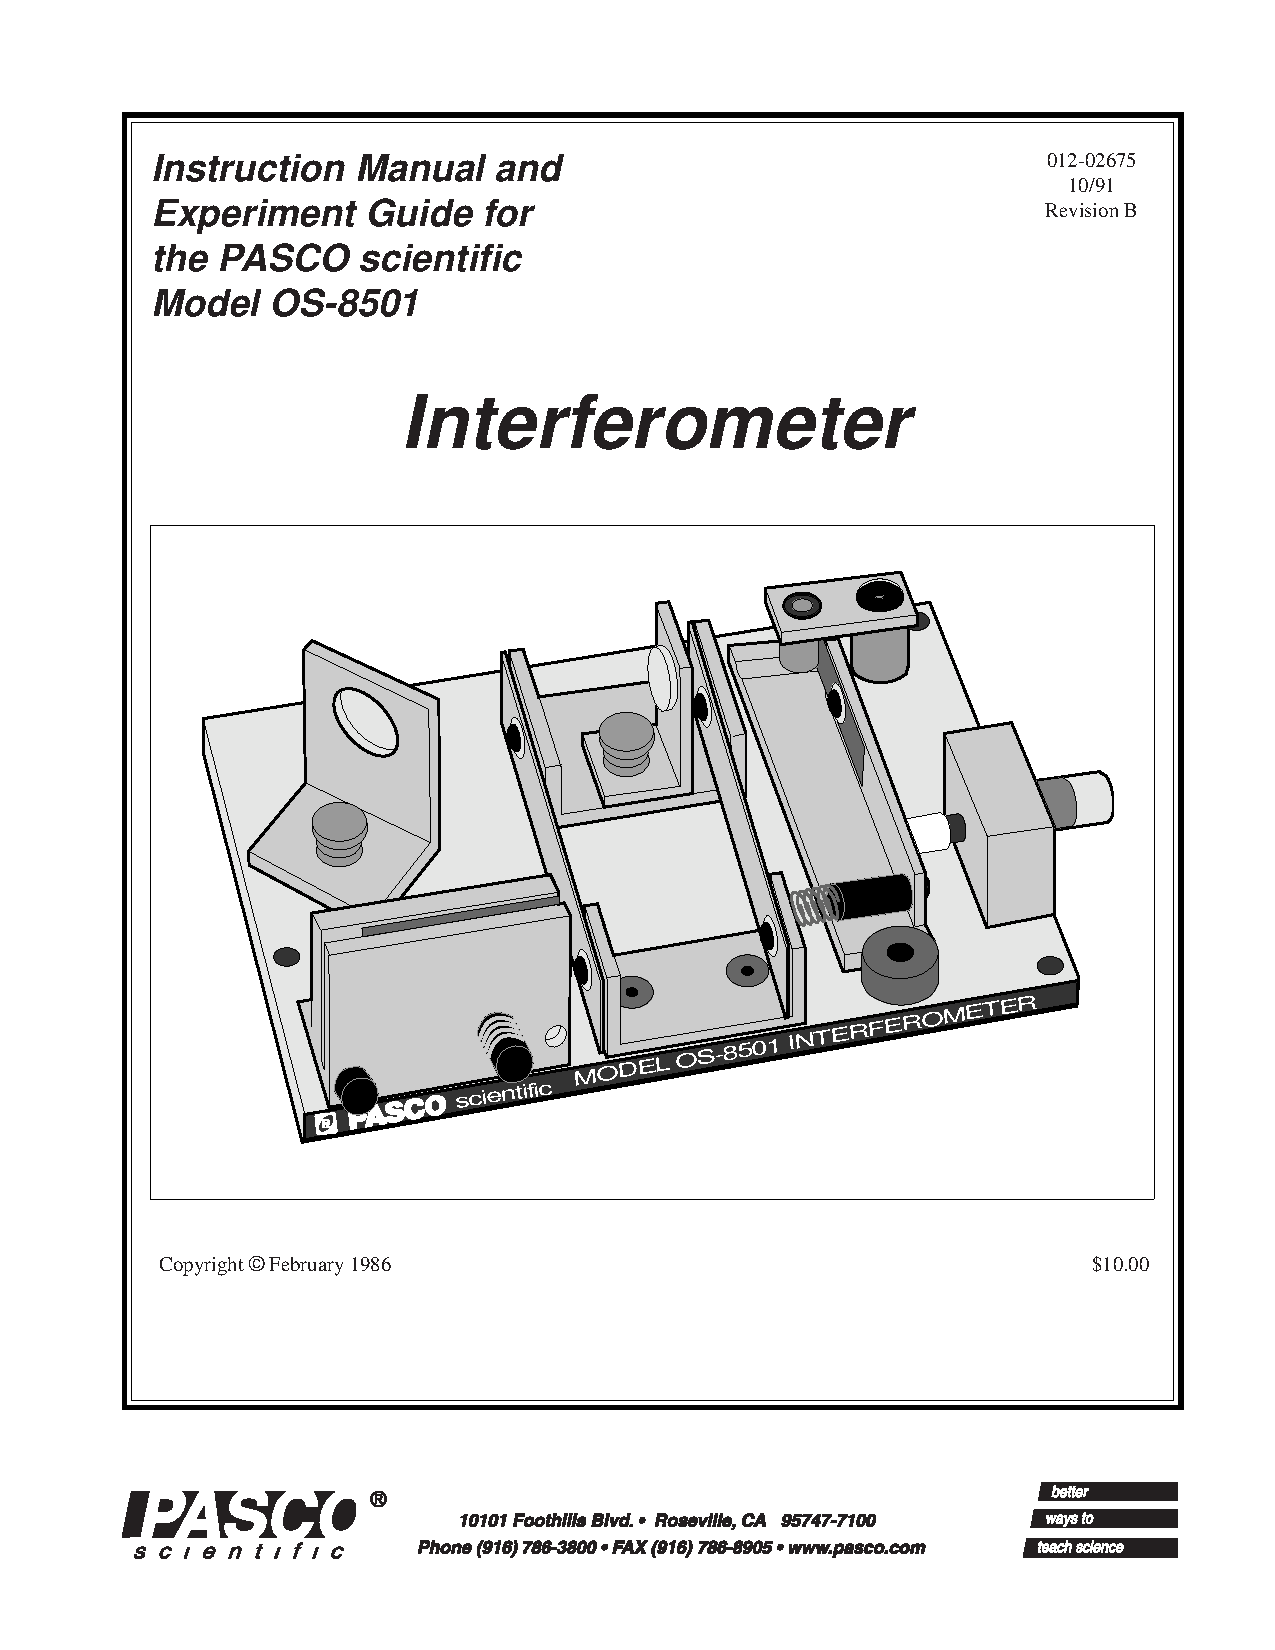
\includepdf[pages={1,6-8}]{pasco-interferometer/Introductory-Michelson-Interferometer-Manual-OS-8501.pdf}

\includepdf[pages={9-10}]{pasco-interferometer/Introductory-Michelson-Interferometer-Manual-OS-8501.pdf}
%\chapter{Manual: PASCO Cavendish Balance}\label{cha:pasco-cavendish}

On the following pages is the manual for the PASCO Cavendish Balance.

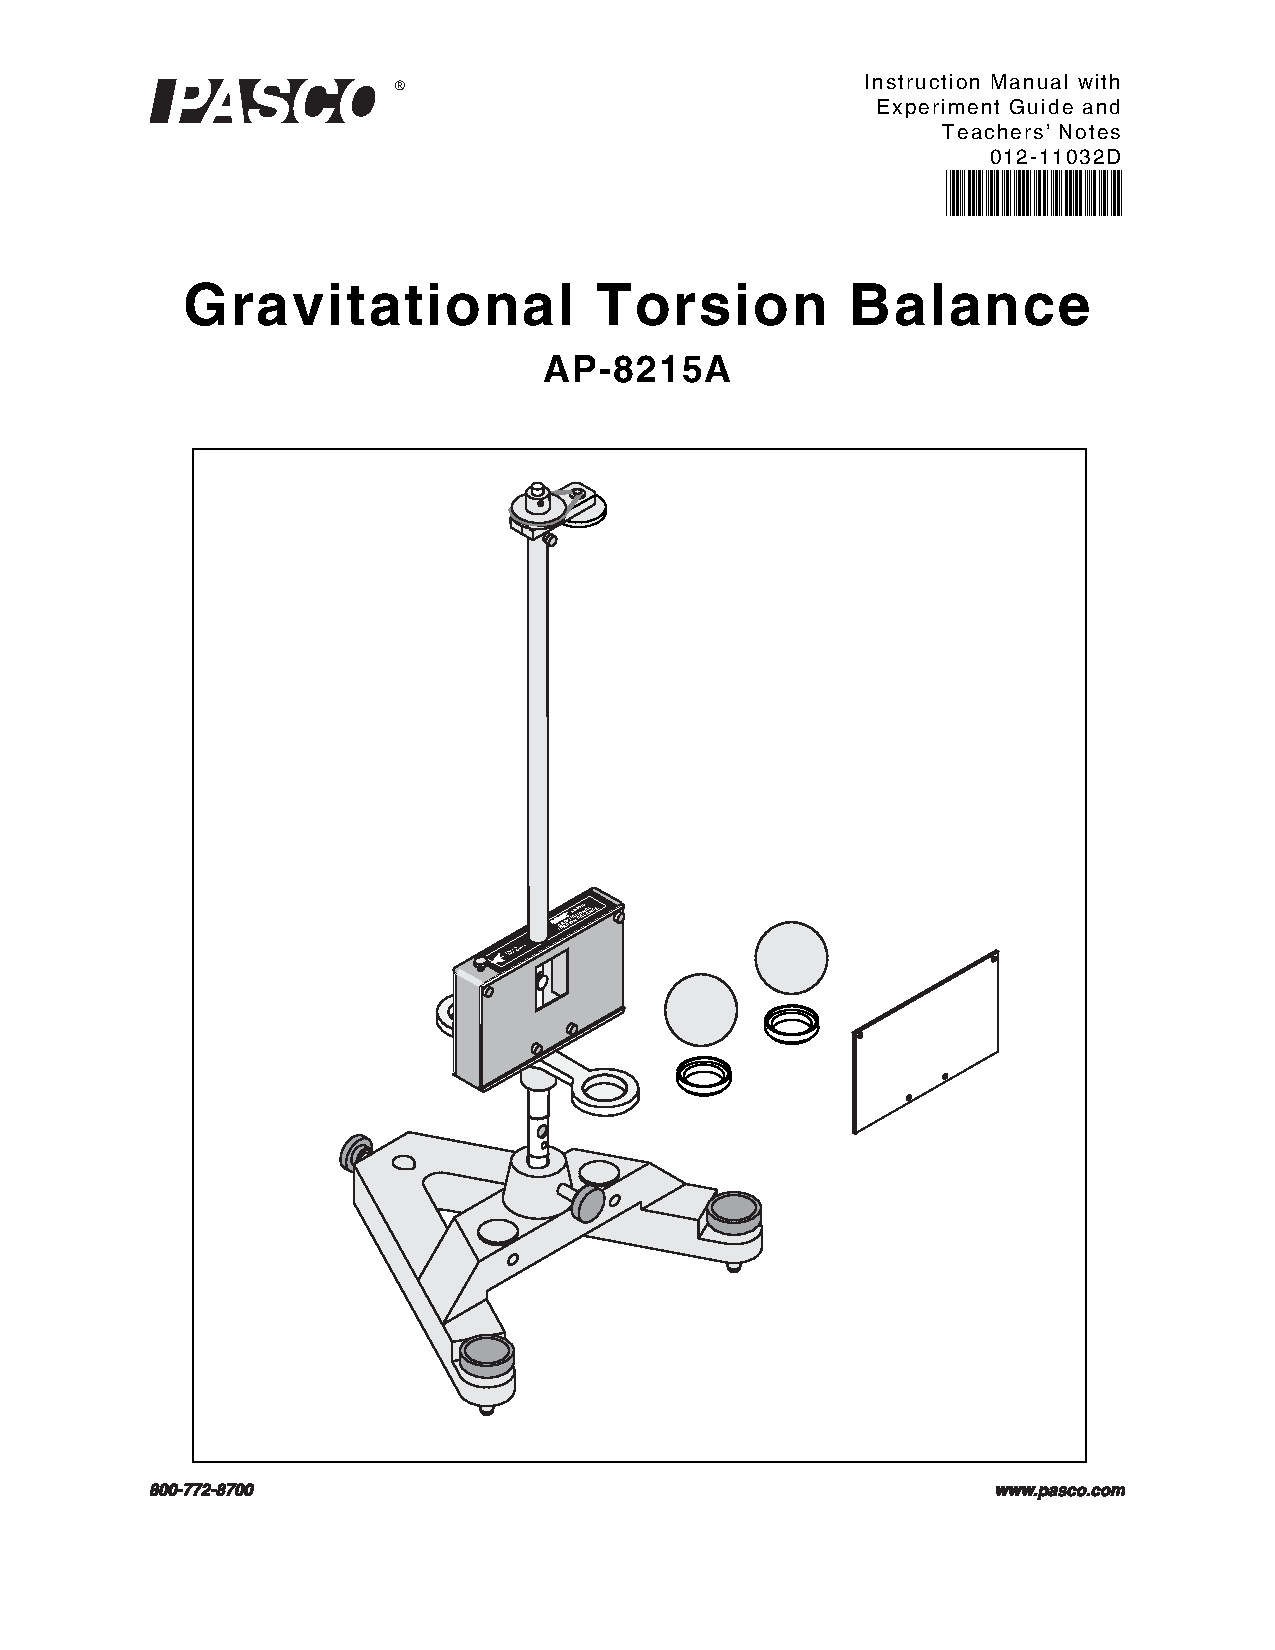
\includepdf[pages={1,3-8,16}]{pasco-cavendish/Gravitational-Torsion-Balance-Manual-AP-8215A.pdf}

% \bibliography{references,MyLibrary}
% \bibliographystyle{plain}
\printbibliography

\end{document}
